%definira klasu dokumenta 
\listfiles
\documentclass[12pt]{report} 

%prostor izmedu naredbi \documentclass i \begin{document} se zove uvod. U njemu se nalaze naredbe koje se odnose na cijeli dokument

%osnovni LaTex ne može riješiti sve probleme, pa se koriste različiti paketi koji olakšavaju izradu željenog dokumenta

\usepackage[utf8]{inputenc}
\usepackage{subcaption}
\usepackage{xcolor}
\usepackage[croatian]{babel} 
\usepackage{amssymb}
\usepackage{amsmath}
\usepackage{txfonts}
\usepackage{mathdots}
\usepackage{titlesec}
\usepackage{array}
\usepackage{lastpage}
\usepackage{etoolbox}
\usepackage{longtable, tabu}
\usepackage{color, colortbl}
\usepackage{adjustbox}
\usepackage{geometry}
\usepackage[classicReIm]{kpfonts}
\usepackage{hyperref}
\usepackage{fancyhdr}

\usepackage{float}
\usepackage{setspace}
\restylefloat{table}


\patchcmd{\chapter}{\thispagestyle{plain}}{\thispagestyle{fancy}}{}{} %redefiniranje stila stranice u paketu fancyhdr

%oblik naslova poglavlja
\titleformat{\chapter}{\normalfont\huge\bfseries}{\thechapter.}{20pt}{\Huge}
\titlespacing{\chapter}{0pt}{0pt}{40pt}


\linespread{1.3} %razmak između redaka

\geometry{a4paper, left=1in, top=1in,}  %oblik stranice

\hypersetup{ colorlinks, citecolor=black, filecolor=black, linkcolor=black,	urlcolor=black }   %izgled poveznice


%prored smanjen između redaka u nabrajanjima i popisima
\newenvironment{packed_enum}{
	\begin{enumerate}
		\setlength{\itemsep}{0pt}
		\setlength{\parskip}{0pt}
		\setlength{\parsep}{0pt}
	}{\end{enumerate}}

\newenvironment{packed_item}{
	\begin{itemize}
		\setlength{\itemsep}{0pt}
		\setlength{\parskip}{0pt}
		\setlength{\parsep}{0pt}
	}{\end{itemize}}


%boja za privatni i udaljeni kljuc u tablicama
\definecolor{LightBlue}{rgb}{0.9,0.9,1}
\definecolor{LightGreen}{rgb}{0.9,1,0.9}


%podesavanje zaglavlja i podnožja

\pagestyle{fancy}
\lhead{Programsko inženjerstvo}
\rhead{$SmartCart$}
\lfoot{$PreljevStoga$}
\cfoot{stranica \thepage/\pageref{LastPage}}
\rfoot{\today}
\renewcommand{\headrulewidth}{0.2pt}
\renewcommand{\footrulewidth}{0.2pt}


\begin{document} 
	
	
	
	\begin{titlepage}
		\begin{center}
			\vspace*{\stretch{1.0}} %u kombinaciji s ostalim \vspace naredbama definira razmak između redaka teksta
			\LARGE Programsko inženjerstvo\\
			\large Ak. god. 2020./2021.\\
			
			\vspace*{\stretch{3.0}}
			
			\huge SmartCart\\
			\Large Dokumentacija, Rev. 1\\
			
			\vspace*{\stretch{12.0}}
			\normalsize
			Grupa: \textit{PreljevStoga}\\
			Voditelj: \textit{Tomislav Bjelčić}\\
			
			
			\vspace*{\stretch{1.0}}
			Datum predaje: \textit{13. studenog 2020.}\\
	
			\vspace*{\stretch{4.0}}
			
			Nastavnik: \textit{dr. sc. Miljenko Krhen}\\
		
		\end{center}

	
	\end{titlepage}

	
	\tableofcontents

	\chapter{Dnevnik promjena dokumentacije}
				
		
		\begin{longtabu} to \textwidth {|X[2, l]|X[13, l]|X[4, l]|X[3, l]|}
			\hline \multicolumn{1}{|l|}{\textbf{Rev.}}	& \multicolumn{1}{l|}{\textbf{Opis promjene/dodatka}} & \multicolumn{1}{|l|}{\textbf{Autori}} & \multicolumn{1}{l|}{\textbf{Datum}} \\[3pt] \hline
			\endfirsthead
			
			\hline \multicolumn{1}{|l|}{\textbf{Rev.}}	& \multicolumn{1}{l|}{\textbf{Opis promjene/dodatka}} & \multicolumn{1}{|l|}{\textbf{Autori}} & \multicolumn{1}{l|}{\textbf{Datum}} \\[3pt] \hline
			\endhead
			
			\hline 
			\endlastfoot
			
			0.1 & Dodan opis zadatka i dio specifikacije. 	& Lakoš & 27.10.2020. 		\\[3pt] \hline 
			0.2	& Prilagođeno i prebačeno u \LaTeX & Grubelić & 4.11.2020. 	\\[3pt] \hline
			0.3	& Dodani arhitektura i dodatak & Grubelić & 8.11.2020. 	\\[3pt] \hline
			0.4	& Dodan dijagram razreda & Vladić, Pranjić & 12.11.2020. 	\\[3pt] \hline
			1.0	& Dovršeno za predaju \LaTeX & Grubelić & 12.11.2020. 	\\[3pt] \hline
			1.1 & Dodana struktura za 2. reviziju i ispitivanje programskog rješenja & Komljenović & 14.1.2021. 	\\[3pt] \hline
			
			
		\end{longtabu}

	\chapter{Opis projektnog zadatka}

    \section{Motivacija}
    Cilj je razviti mobilnu aplikaciju koja će pomoći pri obavljanju kupovine u
    dućanima. Prije odlaska u trgovinu ljudi često pišu popis namirnica koje trebaju
    kupiti. Pritom im je nerijetko bitan ukupan iznos kupovine, a posebno
    ima li željenog proizvoda u trgovini u koju namjeravaju ići. Aplikacija
    „SmartCart” će omogućiti kupcima da sastave
    popis namirnica za kupovinu i izračunati njihovu cijenu na temelju
    podataka o cijenama koje u aplikaciju mogu unijeti trgovci. Popis će imati
    mogućnost pretvaranja u košaricu tijekom kupnje kad se namirnice
    uzimaju s polica, tj. praćenja cijene uzetih namirnica, za one koji se
    ne drže popisa u potpunosti. To će također ubrzati proces kupovine namirnica pa će ljudi manje vremena provoditi u trgovini i bit će manje gužve. Osim toga, trgovcima će to biti odlična promocija jer će oni kupci kojima je svejedno u koju trgovinu idu, moći vidjeti onu s najmanjom cijenom namirnica u blizini. 
    
    \section{Opis rada sustava}
    Budući da je srž aplikacije mogućnost stvaranja popisa, prikaz popisa se otvara i prilikom pokretanja aplikacije. Na popise se mogu dodavati artikli na četiri načina:
    \begin{packed_item}
        \item Skeniranjem barkoda artikla - dodaje se točno određeni artikl zadan barkodom i na popis i u košaricu
        \item Pretragom i odabirom - dodaje se određeni artikl na popis pretragom imena (koja dopušta manje pogreške prilikom unosa)
        \item Zadavanjem filtra - na popisu se nalazi onaj artikl koji najbolje zadovoljava filtar i redukcijsku funkciju (npr. najmanja cijena) u trenutku zadnjeg osvježavanja. Količina dostupnih filtra i redukcijskih funkcija će se mijenjati tijekom razvoja aplikacije. Primjeri funkcija filtra su "Cijena unutar intervala", "Vrsta proizvoda" i "Proizvedeno u", a primjeri redukcijskih funkcija su "Najmanja cijena" i "Najveća cijena po kilogramu"
        \item Dodavanjem iz popisa omiljenih artikala
    \end{packed_item}
    
    Dodanim proizvodima moguće je mijenjati količinu, pregledati informacije ili ih dodati u popis omiljenih artikala, na popisu označenih zvjezdicom, koji se nalazi u bočnoj traci. Svaki se popis sastoji od artikala, njihovih količina i cijena (svaka cijena je povezana s nekom trgovinom). Artikle možemo dodati više puta na isti popis. Korisnik artikle na popisu može označiti dodanima u košaricu. Ukupna cijena košarice, kao i cijena cijelog popisa su prikazane uz popis. Moguće je imati više popisa. Moguća je potpuna manipulacija popisima – stvaranje, brisanje, kopiranje, zatvaranje i otvaranje. Popisi su pohranjeni lokalno na korisničkom uređaju. \\
    
    Budući da svaki trgovac zadaje svoju cijenu za artikle na popisu, postoje tri načina izračuna cijena:
    \begin{packed_item}
        \item Najjeftinija trgovina - korisnik prepušta sustavu da nađe najbližu trgovinu za koju je zbroj cijena svih artikala na popisu najmanji.
        \item Najjeftiniji artikli - korisnik prepušta sustavu da za svaki artikl nađe najbližu trgovinu u kojoj je cijena tog artikla najmanja
        \item Određena trgovina - korisnik pretražuje trgovine i odabire jednu te se cijene osvježe u skladu s time. Ovo je pretpostavljeni način
    \end{packed_item}
    
    Budući da se informacije o trgovinama i cijenama u njima često mijenjaju, korisnik može osvježavati svoje popise. Pritom bojanje oznake količine proizvoda crveno označava da proizvod nije više dostupan u trgovini s kojom je povezan na popisu. Bojanje imena proizvoda crveno označava da proizvod nije više dostupan niti u jednoj trgovini, a bojanje cijene proizvoda crveno ili zeleno označava da se ta cijena redom povećala ili smanjila. \\
    
    Informacije o trgovini moguće je pronaći pritiskom na cijenu artikla u toj trgovini. Tu je moguće pronaći radno vrijeme, adresu, poveznicu za prikaz trgovine na \textit{Google Maps} karti te udaljenost od trgovine ako je dozvoljen pristup lokaciji. \\
    
    Informacije o artiklima i dostupnosti u trgovinama ne spremaju se na uređaju, pa je internetska veza s poslužiteljem nužna za cjelovitu funkcionalnost aplikacije. Aplikacija je u "online" načinu rada ako je povezana s poslužiteljem. Prekidom "online" načina rada aplikacija prelazi u "offline" način rada. Bez veze s poslužiteljem korisnik samo može micati artikle s popisa te stvarati, brisati, otvarati i zatvarati popise bez dodavanja novih artikala. Jedino što je spremljeno u bazi podataka na uređaju su podatci o artiklima na popisima te među omiljenim artiklima. \\
    
    Sva ova funkcionalnost dostupna je neprijavljenom korisniku, tj. \underbar{gostu}. No, potrebno je i nabaviti informacije koje bi se prikazivale u aplikaciji. Neki će pisati korisne infromacije, ali kako bi se zaustavilo one koji bi širili dezinformacije, za upis bilo kakvih informacija potrebno je imati korisnički račun koji administrator prema potrebi može onemogućiti. Neprijavljeni korisnici ne mogu promijeniti informacije o artiklu ni samo na uređaju, kako bi se potaknulo korisnike da podijele podatke koje steknu. \\
    
    Dakle, postoji tri vrste korisnika s korisničkim računom:
    \begin{packed_item}
        \item Kupac
        \item Trgovac
        \item Administrator
    \end{packed_item}
    
    \underbar{Kupac} može, uz osnovnu funkcionalnost koju ima i gost, mijenjati informacije o artiklu, ali samo one koje nisu nužno vezane uz trgovinu. Dakle, opis artikla u pravilu nije vezan uz trgovinu. Samo cijena, popust i dostupnost. Kupac o svim informacijama o artiklu i/ili trgovini može glasati, a na temelju toga se izračunava ocjena pouzdanosti koju vide svi korisnici uz opis. Također, kako bi se povećala vjerojatnost da onaj tko piše informacije o artiklu piše točne podatke, prije spremanja izmijenjenih podataka mora očitati barkod artikla. Za registraciju su mu potrebni samo email i lozinka. \\
    
    \underbar{Trgovac}, uz funkcionalnost kupca, ima i mogućnost dodavanja svojih trgovina te manipulacije njima. Za stvaranje trgovine su mu potrebni lokacija trgovine i radno vrijeme. Trgovac kroz svoju nadzornu ploču na kojoj ima pregled trgovina koje je dodao i proizvoda u njima dodaje ili mijenja artikle kao petorku (barkod, cijena, popust, dostupnost, email adresa željenog opisivača). Barkod je potreban da bi korisnici znali da je taj proizvod u toj trgovini, cijena i popust određuju ukupnu cijenu proizvoda koja će pisati na popis, a dostupnost označava ima li artikla u trgovini bez da ga se briše. Trgovac ne mora unositi opis artikla, ali ako postavi email adresu željenog opisivača i korisnik s tom email adresom je napisao opis o artiklu s tim barkodom, taj opis nadjača ostale kad se prikazuje cijena artikla u toj trgovini. Inače se informacije o artiklu u trgovini povezuju s najpouzdanijim opisom. Nove informacije o artiklima se mogu učitati i iz csv datoteke jednakog rasporeda stupaca. Kako bi se smanjila vjerojatnost lažnog predstavljanja i neispravnih informacija o cijenama i dostupnosti artikala u trgovini, trgovac za registraciju mora upisati tajni broj koji je dobio (uživo) od administratora i samo on smije mijenjati informacije o trgovinama. Tu je ipak novac "u igri". \\
    
    \underbar{Administrator} ima zadaću održavati red u sustavu. Može vidjeti sve podatke (poput broja glasova na opisima trgovaca i kupaca te njihovih mail adresa, lozinke su sakrivene SHA-256 algoritmom), a mijenjati može informacije o artiklima, kao i kupac. Može onemogućiti pristup bilo kojem korisničkom računu, uključujući trgovce i druge administratore (za micanje privilegija administratoru ipak treba najmanje pola glasova administratora u istom danu). Trgovcu, iako ne može mijenjati informacije o trgovini, može ukloniti trgovinu kako bi se ipak spriječilo zlonamjerno iskorištavanje sustava. Administrator također privilegije stiče registracijom uz tajni broj koji dobije (uživo) od drugih administratora. \\
    
    \section{Mogućnosti proširenja}
    
    Iako je aplikacija u ovom obliku potpuno funkcionalna, ako preraste u pravi proizvod postoji više mogućnosti proširenja i poboljšanja korisničkog iskustva:
    \begin{packed_item}
        \item Proširenje mogućnosti korištenja u načinu rada bez veze s poslužiteljem
        \item Slike artikala
        \item API za trgovce i/ili kupce
        \item Spremanje popisa u bazu na poslužitelju
        \item Dijeljenje popisa
        \item Praćenje cijene artikala kroz vrijeme
        \item Tlocrt trgovina i promjena poretka artikala na popisu
        \item Podržavanje popusta vezanih uz kartice vjernosti
        \item Posredovanje u "online" kupovini
        \item Suradnja sa stranicom poput Coolinarike za ubacivanje sastojaka jela na korisnički popis
        \item Definiranje maksimalnog broja trgovina po kojima se podijele sastojci iz košarice za izračun minimalne cijene (trenutno postoje dvije krajnosti: 1 i broj artikala)
    \end{packed_item}
    
    
    \section{Slične aplikacije}
    
    U nastavku su navedene dvije aplikacije čija je funkcionalnost slična onoj naše aplikacije. Ipak, valja naglasiti da nam one nisu ni inspiracija niti ih nastojimo imitirati. One su upravo to - aplikacije s nekim funkcionalnostima sličnima našoj.
    
    \subsection{SmartCart: Shopping list}
    
    Ova aplikacija (\ref{fig:SmartCart: Shopping list}) je slična našoj po tome što ima funkcionalnost stvaranja više popisa i manipulacije njima. Bitna razlika je to što nema "agregator cijena" nego sve cijene upisuje korisnik. Za ovu aplikaciju smo saznali tek nakon definiranja specifikacije programske potpore, nakon pretrage trgovine \textit{Google Play} za potrebe ove dokumentacije, zato ima vrlo slično ime i neke detalje jer izgleda da slično razmišljamo.
    
    \begin{figure}
        \centering
        \begin{subfigure}{0.49\textwidth}
            \centering
            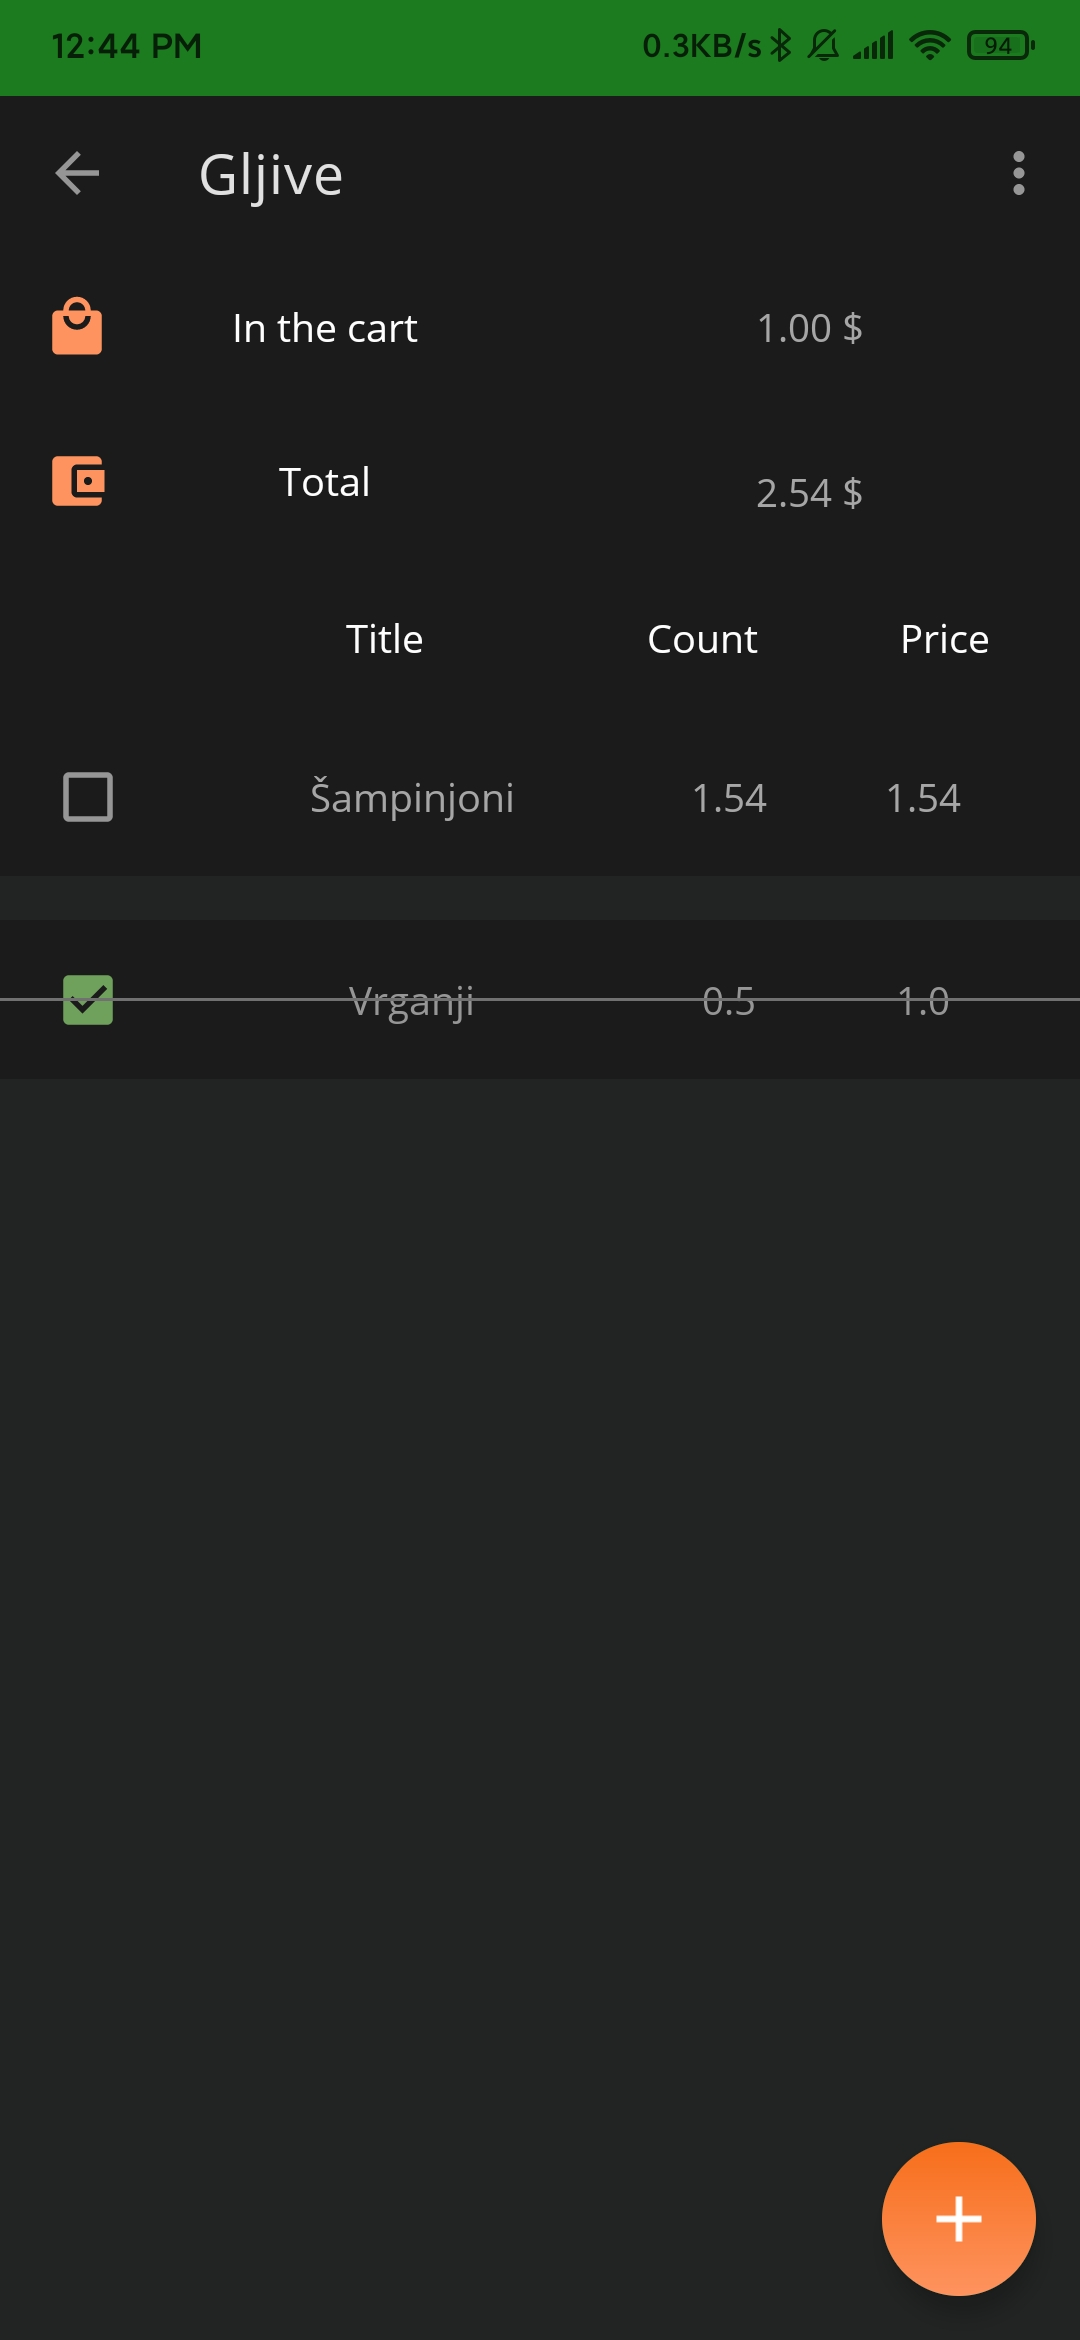
\includegraphics[width = \textwidth]{slike/Informerlab.jpg}
            \caption{SmartCart:Shopping list}
            \label{fig:SmartCart: Shopping list}
        \end{subfigure}
        \begin{subfigure}{0.49\textwidth}
            \centering
            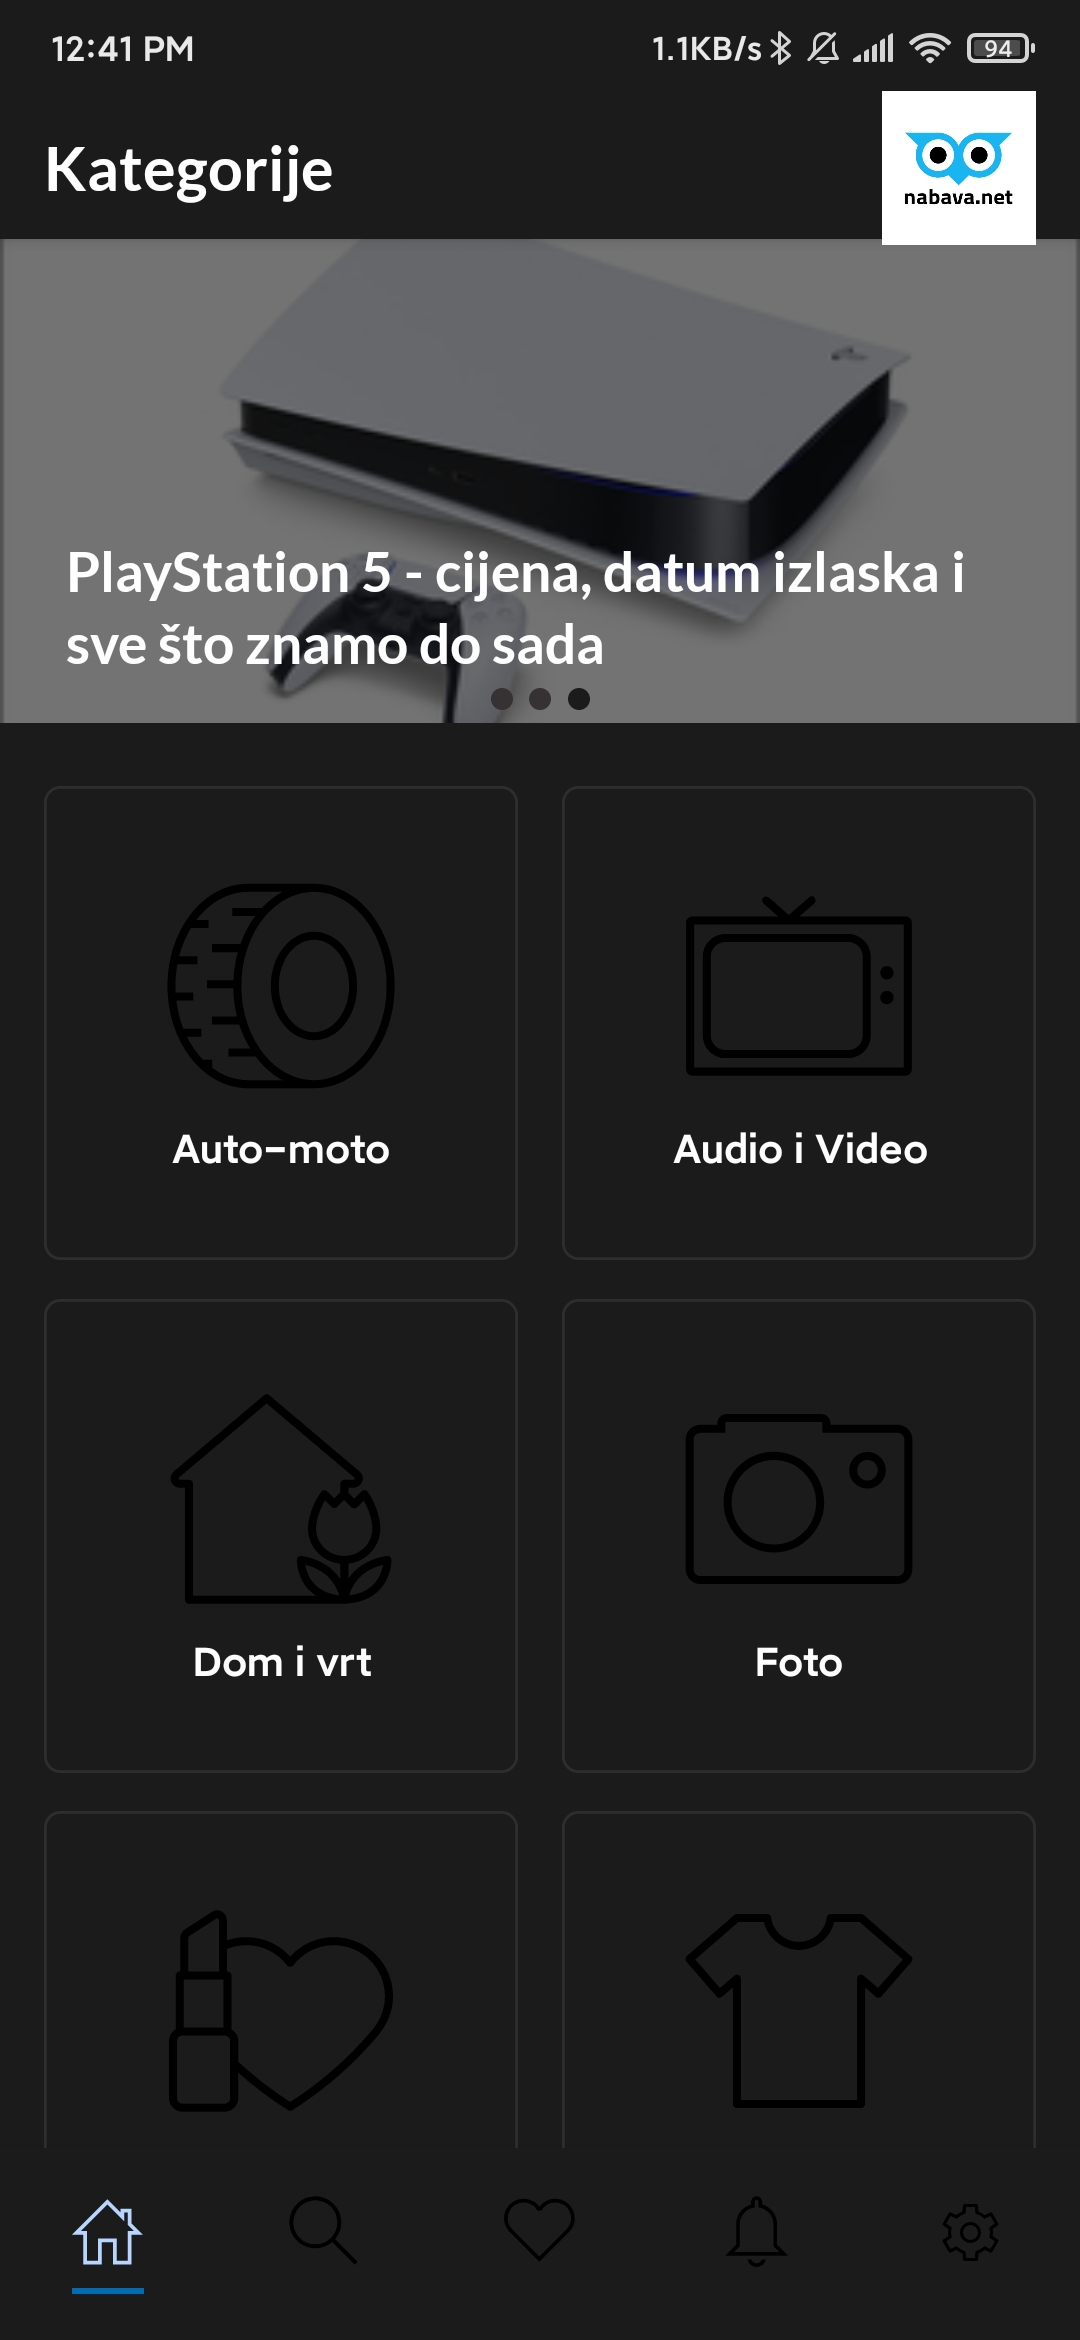
\includegraphics[width = \textwidth]{slike/nabava_net.jpg}
            \caption{nabava.net}
            \label{fig:nabava.net}
        \end{subfigure}
        % \label{fig:combined}
    \end{figure}
    
    
    \subsection{nabava.net}
    
    Aplikacija nabava.net (\ref{fig:nabava.net}) ima upravo suprotno - "agregator cijena", ali nema košaricu i usredotočena je na "online" kupovinu. Nije toliko usredotočena na namirnice. Mobilna aplikacija joj je zapravo prilagodba web aplikacije.
    
        
        \eject
        
    

	\chapter{Specifikacija programske potpore}
		
	\section{Funkcionalni zahtjevi}
		
			\noindent \textbf{Dionici:}
			
			\begin{packed_enum}
				
				\item Neprijavljeni korisnici
				\item Kupci	
				\item Trgovci
				\item Administratori (nadskup razvojnog tima)
				
			\end{packed_enum}
			
			\noindent \textbf{Aktori i njihovi funkcionalni zahtjevi:}
			
			
			\begin{packed_enum}
				\item  \underbar{Neprijavljeni korisnik, tj. gost (inicijator) može:}
				
				\begin{packed_enum}
					
					\item vidjeti trgovine u blizini (TuB) kao popis
					\item prikazati TuB na karti
					\item odabrati TuB kao željenu za prikaz dostupnosti i cijena artikala
					\item vidjeti za svaki artikl s popisa posebno u kojoj je TuB najjeftiniji
					\item vidjeti za cijelu košaricu u kojoj TuB je dostupna i najjeftinija
					\item upravljati popisima
					\begin{packed_enum}
						
						\item stvarati nove popise
						\item preimenovati popise
						\item odabrati koji popis se prikazuje
						\item pretraživati artikle i dodavati ih na prikazani popis
						\item micati artikle s prikazanog popisa
						\item sve artikle s prikazanog popisa kopirati na neki drugi
						\item obrisati prikazani popis
						\item označiti artikle kao dodane u košaricu 
				
					\end{packed_enum}
					\item označiti artikl kao omiljeni za lakši pristup
					\item vidjeti mjeru pouzdanosti informacija o artiklu
					\item vidjeti ukupnu cijenu popisa
					\item vidjeti cijenu košarice
					\begin{packed_enum}
					    \item prijaviti se u sustav
					    \item registrirati se u sustav, stvoriti korisnički račun za koji su mu potrebni e-mail adresa i lozinka ili Google račun
					    \item promijeniti lozinku
					\end{packed_enum}
					
				\end{packed_enum}
				
			\item \underbar{Kupac (inicijator) može:}
				
				\begin{packed_enum}
					
					\item sve što može i neprijavljeni korisnik osim prijave
					\item glasati o ispravnosti informacija o artiklu
					\item uz skeniranje artikla napisati informacije o njemu ako su trenutne neispravne ili ih nema
					\item obrisati račun
					\item promijeniti lozinku
				\end{packed_enum}
			
			\item \underbar{Trgovac (inicijator) može:}
				
				\begin{packed_enum}
					
					\item sve što može i kupac, samo mu je za registraciju potreban dodatni verifikacijski kôd
					\item upravljati svojim trgovinama
					\begin{packed_enum}
						
						\item stvarati nove trgovine (potrebno navesti lokaciju i radno vrijeme)
						\item obrisati postojeće trgovine
						\item u bilo koju trgovinu dodati artikle s pripadnim cijenama
						\item mijenjati cijene artikala
						\item označiti da su artikli na popustu
						\item označiti da je neki artikl rasprodan
						\item maknuti artikl iz trgovine
						\item mijenjati radno vrijeme trgovine
					\end{packed_enum}
				\end{packed_enum}
			
			\item \underbar{Administrator (inicijator) može:}
				
				\begin{packed_enum}
					
					\item sve što može i kupac, samo mu je za registraciju potreban dodatni verifikacijski kôd
					\item pristupiti administratorskoj nadzornoj ploči preko web-sučelja
					\item ukloniti korisnika
					\item ukloniti trgovinu
				\end{packed_enum}
			
			
				\item \underbar{Baza podataka na poslužitelju (sudionik):}
				
				\begin{packed_enum}
					
					\item pohranjuje sve podatke o sudionicima i njihovim ovlastima
					\item pohranjuje sve podatke o artiklima
					\item pohranjuje sve podatke o trgovinama
					
				\end{packed_enum}
				
				\item \underbar{Baza podataka na uređaju (sudionik):}
				
				\begin{packed_enum}
					
					\item pohranjuje podatke o popisima i omiljenim artiklima korisnika
					
				\end{packed_enum}
				
				\item \underbar{Email poslužitelj (sudionik):}
				
				\begin{packed_enum}
					
					\item šalje privremenu lozinku korisniku koji je zaboravio svoju
					\item šalje obavijesti administratorima (o onemogućavanju pristupa jednom od njih)
					
				\end{packed_enum}
			\end{packed_enum}
			
			\eject 
			
			
				
			\subsection{Obrasci uporabe}

				\subsubsection{Opis obrazaca uporabe}
			
				
				\noindent \underbar{\textbf{UC0 - Postavljanje najveće udaljenosti}}
				\begin{packed_item}
					\item \textbf{Glavni sudionik:} Korisnik
					\item  \textbf{Cilj:} Ograničiti polumjer u kojem mogu biti rezultati pretrage trgovine
					\item  \textbf{Sudionici:} Baza podataka na poslužitelju
					\item  \textbf{Preduvjet:} Dozvoljen je pristup lokaciji
					\item  \textbf{Opis osnovnog tijeka:}
					\item[] \begin{packed_enum}
						\item Korisnik otvara postavke aplikacije
						\item Korisnik postavlja najveću udaljenost unutar koje može biti rezultat pretrage. Udaljenost se računa kao euklidska udaljenost geografske širine i dužine
						\item Ubuduće prilikom svakog upita vezanog uz trgovine osim ručne pretrage baza prvo odstrani one koje su dalje od najveće dopuštene udaljenosti od korisnika ako je pristup lokaciji još uvijek dozvoljen
					\end{packed_enum}
					\item  \textbf{Opis mogućih odstupanja:}
					\item[] \begin{packed_item}
						\item[3.a] Korisnik makne dozvolu pristupa lokaciji u nekom trenutku
						\item[] \begin{packed_enum}
							\item Ne primjenjuje se ograničenje na lokaciju trgovine 
						\end{packed_enum}
					\end{packed_item}
					\item  \textbf{Opis mogućih odstupanja:}
					\item[] \begin{packed_item}
						\item[3.b] Korisnik je na polu ili najkraći put do trgovine prelazi meridijan $\pm{180}$
						\item[] \begin{packed_enum}
							\item Korisnik potencijalno dobiva pogrešne rezultate, ali ih svi dobivaju brzo
						\end{packed_enum}
					\end{packed_item}
				\end{packed_item}
					
				%1 Stvaranje popisa
				\noindent \underbar{\textbf{UC1 - Stvaranje popisa}}
				\begin{packed_item}
					\item \textbf{Glavni sudionik:} Korisnik
					\item \textbf{Cilj:} Stvoriti novi popis artikala
					\item \textbf{Sudionici:} Baza podataka na uređaju
					\item \textbf{Preduvjet:} -
					\item \textbf{Opis osnovnog tijeka:}
					\item[] \begin{packed_enum}
						\item korisnik otvori izbornik
						\item odabere opciju "Stvori novi popis"
						\item na mjesto prikazanog popisa se stavlja novi prazni popis s pretpostavljenim imenom "Novi popis"
					\end{packed_enum}
				\end{packed_item}
				
					
				\noindent \underbar{\textbf{UC2 - Otvaranje drugog popisa}}
				\begin{packed_item}
					\item \textbf{Glavni sudionik:} Korisnik
					\item  \textbf{Cilj:} Prikazivanje određenog postojećeg popisa
					\item  \textbf{Sudionici:} Baza podataka na uređaju
					\item  \textbf{Preduvjet:} Postoji više od jednog popisa
					\item  \textbf{Opis osnovnog tijeka:}
					\item[] \begin{packed_enum}
						\item Korisnik otvori izbornik sa svim popisima
						\item Korisnik odabire popis s izbornika
						\item Drugi popis zamijenjuje prikazani
					\end{packed_enum}
					\item  \textbf{Opis mogućih odstupanja:}
					\item[] \begin{packed_item}
						\item[1.a] Nema drugih popisa
						\item[] \begin{packed_enum}
							\item Korisnik dobije obavijest da nema drugih popisa i ne otvara se izbornik
						\end{packed_enum}
					\end{packed_item}
				\end{packed_item}
				
					
				\noindent \underbar{\textbf{UC3 - Brisanje popisa}}
				\begin{packed_item}
					\item \textbf{Glavni sudionik:} Korisnik
					\item  \textbf{Cilj:} Obrisati popis
					\item  \textbf{Sudionici:} Baza podataka na uređaju
					\item  \textbf{Preduvjet:} -
					\item  \textbf{Opis osnovnog tijeka:}
					\item[] \begin{packed_enum}
						\item Korisnik otvara popis koji želi obrisati
						\item Korisnik pritisne gumb za brisanje
						\item Korisnik potvrdi da želi obrisati popis
						\item Popis se briše i prikazuje se drugi
					\end{packed_enum}
					\item  \textbf{Opis mogućih odstupanja:}
					\item[] \begin{packed_item}
						\item[4.a] Ne postoji drugi popis
						\item[] \begin{packed_enum}
							\item Stvara se novi prazni popis
						\end{packed_enum}
					\end{packed_item}
				\end{packed_item}
				
					
				\noindent \underbar{\textbf{UC4 - Preimenovanje popisa}}
				\begin{packed_item}
					\item \textbf{Glavni sudionik:} Korisnik
					\item  \textbf{Cilj:} Preimenovanje popisa
					\item  \textbf{Sudionici:} Baza podataka na uređaju
					\item  \textbf{Preduvjet:} -
					\item  \textbf{Opis osnovnog tijeka:}
					\item[] \begin{packed_enum}
						\item Korisnik dugo pritisne ime otvorenog popisa
						\item Otvori se prikaz za upis teksta
						\item Izlaskom iz prikaza se sadržaj spremi kao novo ime popisa
					\end{packed_enum}
				\end{packed_item}
			
				
				\noindent \underbar{\textbf{UC5 - Kopiranje sadržaja popisa}}
				\begin{packed_item}
					\item \textbf{Glavni sudionik:} Korisnik
					\item  \textbf{Cilj:} Sve podatke s popisa nadodati na kraj drugog popisa
					\item  \textbf{Sudionici:} Baza podataka na uređaju
					\item  \textbf{Preduvjet:} Postojanje dva popisa (predložak i odredište)
					\item  \textbf{Opis osnovnog tijeka:}
					\item[] \begin{packed_enum}
						\item Korisnik otvara popis predložak
						\item Korisnik pritisne gumb "kopiraj"
						\item Otvara se izbornik popisa
						\item Korisnik odabire popis s izbornika
						\item Svi artikli i njihove količine se dodaju na kraj popisa odredište
					\end{packed_enum}
					\item  \textbf{Opis mogućih odstupanja:}
					\item[] \begin{packed_item}
						\item[3.a] Popis odredište ne postoji
						\item[] \begin{packed_enum}
							\item Korisnik dobije obavijest da nema drugih popisa i ne otvara se izbornik
						\end{packed_enum}
					\end{packed_item}
				\end{packed_item}
				
				%6 Dodavanje artikla - Barkod
				\noindent \underbar{\textbf{UC6 - Dodavanje artikla na popis pomoću barkoda}}
					\begin{packed_item}
						\item \textbf{Glavni sudionik:} Korisnik
						\item  \textbf{Cilj:} Dodati određeni artikl na popis i u košaricu
						\item  \textbf{Sudionici:} Baza podataka na uređaju, baza podataka na poslužitelju
						\item  \textbf{Preduvjet:} Veza s poslužiteljem
						\item  \textbf{Opis osnovnog tijeka:}
						\item[] \begin{packed_enum}
							\item Korisnik pritisne gumb za dodavanje artikla na popis pomoću barkoda
							\item Korisnik skenira barkod
							\item Baza na poslužitelju vrati informacije o artiklu povezanom s barkodom
							\item Artikl se doda na kraj popisa i u košaricu, pretpostavljena količina je 1
						\end{packed_enum}
						\item  \textbf{Opis mogućih odstupanja:}
						\item[] \begin{packed_item}
							\item[2.a] Korisnik ne može pristupiti kameri, tj. barkod skeneru
							\item[] \begin{packed_enum}
								\item Sustav korisniku omogućava ručni upis znamenaka
							\end{packed_enum}
							\item[3.a] Nema informacija o artiklu u bazi podataka na poslužitelju
							\item[] \begin{packed_enum}
							    \item Upisuje se samo cijena ako postoji, inače se ispisuje poruka suosjećanja
							\end{packed_enum}
						\end{packed_item}
					\end{packed_item}
				
					
				\noindent \underbar{\textbf{UC7 - Dodavanje artikla na popis pretragom}}
				\begin{packed_item}
					\item \textbf{Glavni sudionik:} Korisnik
					\item  \textbf{Cilj:} Dodati određeni artikl na popis
					\item  \textbf{Sudionici:} Baza podataka na uređaju, baza podataka na poslužitelju
					\item  \textbf{Preduvjet:} Veza s poslužiteljem
					\item  \textbf{Opis osnovnog tijeka:}
					\item[] \begin{packed_enum}
						\item Korisnik pritisne gumb za dodavanje artikla na popis pretragom
						\item Korisnik upisuje naziv artikla
						\item Korisnik odabire jedan od ponuđenih artikala
						\item Artikl se doda na kraj popisa, pretpostavljena količina je 1
					\end{packed_enum}
					\item  \textbf{Opis mogućih odstupanja:}
					\item[] \begin{packed_item}
						\item[3.a] Nema traženog artikla
						\item[] \begin{packed_enum}
							\item Ispisuje se poruka suosjećanja na mjestu gdje bi trebali biti rezultati pretrage
						\end{packed_enum}
					\end{packed_item}
				\end{packed_item}
				
					
				\noindent \underbar{\textbf{UC8 - Dodavanje artikla na popis zadavanjem filtra}}
				\begin{packed_item}
					\item \textbf{Glavni sudionik:} Korisnik
					\item  \textbf{Cilj:} Dodati na popis artikl koji zadovoljava filter
					\item  \textbf{Sudionici:} Baza podataka na uređaju, baza podataka na poslužitelju
					\item  \textbf{Preduvjet:} Veza s poslužiteljem
					\item  \textbf{Opis osnovnog tijeka:}
					\item[] \begin{packed_enum}
						\item Korisnik pritisne gumb za dodavanje artikla na popis pomoću filtra
						\item Korisnik postavlja filter i/ili redukciju (min, max)
						\item Artikl koji zadovoljava filter se doda na kraj popisa, pretpostavljena količina je 1
					\end{packed_enum}
					\item  \textbf{Opis mogućih odstupanja:}
					\item[] \begin{packed_item}
						\item[3.a] Više artikala zadovoljava filtar i/ili redukciju
						\item[] \begin{packed_enum}
							\item Odabire se onaj s najnižom cijenom koji je najbliži ako je dozvoljen pristup lokaciji, inače prvi u bazinom odgovoru na upit
						\end{packed_enum}
					\end{packed_item}
				\end{packed_item}
				
					
				\noindent \underbar{\textbf{UC9 - Dodavanje artikla iz popisa omiljenih artikala}}
				\begin{packed_item}
					\item \textbf{Glavni sudionik:} Korisnik
					\item  \textbf{Cilj:} Dodati na popis artikl iz popisa omiljenih artikala
					\item  \textbf{Sudionici:} Baza podataka na uređaju
					\item  \textbf{Preduvjet:} Postoji omiljeni artikl
					\item  \textbf{Opis osnovnog tijeka:}
					\item[] \begin{packed_enum}
						\item Korisnik otvori bočnu traku
						\item Korisnik pritisne željeni artikl
						\item Artikl se doda na kraj popisa, pretpostavljena količina je 1
						\item Popis se osvježi
					\end{packed_enum}
				\end{packed_item}
			
				
				\noindent \underbar{\textbf{UC10 - Zamjena artikla na popisu nekim drugim artiklom}}
				\begin{packed_item}
					\item \textbf{Glavni sudionik:} Korisnik
					\item  \textbf{Cilj:} Zamijeniti artikl na popisu nekim drugim artiklom
					\item  \textbf{Sudionici:} Baza podataka na uređaju, baza podataka na poslužitelju
					\item  \textbf{Preduvjet:} Postoji artikl na popisu, veza s poslužiteljem
					\item  \textbf{Opis osnovnog tijeka:}
					\item[] \begin{packed_enum}
						\item Korisnik povuče artikl na popisu ulijevo
						\item Korisnik odabire novi artikl na onaj način na koji je dodan stari artikl
						\item Novi artikl je prikazan na mjestu starog, pretpostavljena količina je 1
					\end{packed_enum}
				\end{packed_item}
			
				
				\noindent \underbar{\textbf{UC11 - Micanje artikla s popisa}}
				\begin{packed_item}
					\item \textbf{Glavni sudionik:} Korisnik
					\item  \textbf{Cilj:} U potpunosti maknuti artikl s popisa
					\item  \textbf{Sudionici:} Baza podataka na uređaju
					\item  \textbf{Preduvjet:} Postoji artikl na popisu
					\item  \textbf{Opis osnovnog tijeka:}
					\item[] \begin{packed_enum}
						\item Korisnik povuče artikl na popisu udesno
						\item Artikl se miče s popisa
					\end{packed_enum}
				\end{packed_item}
			
				
				\noindent \underbar{\textbf{UC12 - Registracija korisnika}}
				\begin{packed_item}
					\item \textbf{Glavni sudionik:} Gost
					\item  \textbf{Cilj:} Stvaranje korisničkog računa
					\item  \textbf{Sudionici:} Baza podataka na poslužitelju
					\item  \textbf{Preduvjet:} Veza s poslužiteljem
					\item  \textbf{Opis osnovnog tijeka:}
					\item[] \begin{packed_enum}
						\item Gost otvara izbornik
						\item Gost u izborniku odabire "Registracija"
						\item Gost upisuje email, lozinku i potvrdu lozinke za registraciju kao kupac. Dodatno tajni broj za registraciju kao trgovac ili administrator
						\item Baza provjerava postoji li već korisnik s istom adresom elektroničke pošte
						\item Korisnik dobiva povratnu informaciju
					\end{packed_enum}
					\item  \textbf{Opis mogućih odstupanja:}
					\item[] \begin{packed_item}
						\item[3.a] Email adresa je u neispravnom obliku, lozinka ima manje od 8 znakova ili se potvrda ne podudara
						\item[] \begin{packed_enum}
							\item Korisnik dobiva odgovarajuću informativnu poruku, podatci se ne brišu ni ne šalju
						\end{packed_enum}
						\item[4.a] U bazi već postoji korisnikova mail adresa
						\item[] \begin{packed_enum}
							\item Korisnik dobiva odgovarajuću informativnu poruku, podatci se ne brišu
						\end{packed_enum}
					\end{packed_item}
				\end{packed_item}
			
				
				\noindent \underbar{\textbf{UC13 - Prijava korisnika}}
				\begin{packed_item}
					\item \textbf{Glavni sudionik:} Gost
					\item  \textbf{Cilj:} Prijava u sustav
					\item  \textbf{Sudionici:} Baza podataka na poslužitelju, email poslužitelj u slučaju odstupanja 2.a
					\item  \textbf{Preduvjet:} Veza s poslužiteljima (sustav, baza podataka i email), gost ima račun
					\item  \textbf{Opis osnovnog tijeka:}
					\item[] \begin{packed_enum}
						\item Gost otvara sučelje za prijavu
						\item Gost upisuje email adresu i lozinku ili se prijavi pomoću Google računa
						\item Baza podataka provjerava dane informacije
						\item Gost dobije povratnu informaciju
					\end{packed_enum}
					\item  \textbf{Opis mogućih odstupanja:}
					\item[] \begin{packed_item}
						\item[2.a] Korisnik ne zna koju lozinku ima ili više ne želi koristiti postojeću
						\item[] \begin{packed_enum}
							\item Korisnik pritisne gumb "Promijeni lozinku"
							\item Korisnik upiše svoju mail adresu
							\item Sustav preko email poslužitelja šalje poruku s privremenom lozinkom koju sprema u bazu
							\item Korisnik dobiva novu lozinku na mail adresu
							\item Korisnik se prijavi u aplikaciju i promijeni lozinku (UC15)
						\end{packed_enum}
					    \item[3.a] Email adresa je u neispravnom obliku ili lozinka ima manje od 8 znakova
						\item[] \begin{packed_enum}
							\item Korisnik dobiva odgovarajuću informativnu poruku, podatci se ne brišu ni ne šalju
						\end{packed_enum}
						\item[3.b] U bazi ne postoji korisnikova mail adresa s pripadnom lozinkom ili je račun označen kao onemogućen
						\item[] \begin{packed_enum}
							\item Korisnik dobiva odgovarajuću informativnu poruku
						\end{packed_enum}
					\end{packed_item}
				\end{packed_item}
			
				
				\noindent \underbar{\textbf{UC14 - Odjava korisnika}}
				\begin{packed_item}
					\item \textbf{Glavni sudionik:} Prijavljeni korisnik (kupac, trgovac ili administrator)
					\item  \textbf{Cilj:} Prijeći u način rada neprijavljenog korisnika
					\item  \textbf{Sudionici:} Baza podataka na poslužitelju
					\item  \textbf{Preduvjet:} Veza s poslužiteljem, korisnik je prijavljen
					\item  \textbf{Opis osnovnog tijeka:}
					\item[] \begin{packed_enum}
						\item Prijavljeni korisnik otvara izbornik
						\item Prijavljeni korisnik u izborniku odabire "Odjava"
						\item Korisnik je odjavljen
					\end{packed_enum}
				\end{packed_item}
				
			
				
				\noindent \underbar{\textbf{UC15 - Promjena lozinke}}
				\begin{packed_item}
					\item \textbf{Glavni sudionik:} Prijavljeni korisnik
					\item  \textbf{Cilj:} Promijeniti lozinku 
					\item  \textbf{Sudionici:} Baza podataka na poslužitelju
					\item  \textbf{Preduvjet:} Veza s poslužiteljem, korisnik je prijavljen email adresom i lozinkom
					\item  \textbf{Opis osnovnog tijeka:}
					\item[] \begin{packed_enum}
						\item Prijavljeni korisnik otvara izbornik
						\item Prijavljeni korisnik u izborniku odabire "Promjena lozinke"
						\item Prijavljeni korisnik upiše staru lozinku, novu lozinku i potvrdu nove lozinke
						\item Prijavljeni korisnik dobiva obavijest o uspješnoj promjeni lozinke
					\end{packed_enum}
					\item  \textbf{Opis mogućih odstupanja:}
					\item[] \begin{packed_item}
						\item[3.a] Korisnikova trenutna lozinka nije ispravna ili se potvrda nove lozinke ne podudara
						\item[] \begin{packed_enum}
							\item Korisnik dobiva odgovarajuću informativnu poruku
						\end{packed_enum}
					\end{packed_item}
				\end{packed_item}
			
				
				\noindent \underbar{\textbf{UC16 - Pregled informacija o artiklu}}
				\begin{packed_item}
					\item \textbf{Glavni sudionik:} Korisnik
					\item  \textbf{Cilj:} Pregledati informacije o artiklu
					\item  \textbf{Sudionici:} Baza podataka na poslužitelju
					\item  \textbf{Preduvjet:} Veza s poslužiteljem i artikl na popisu
					\item  \textbf{Opis osnovnog tijeka:}
					\item[] \begin{packed_enum}
						\item Korisnik pritisne ime ili cijenu artikla na popisu
						\item Korisniku se prikažu informacije o artiklu i mjera pouzdanosti tih informacija
					\end{packed_enum}
				\end{packed_item}
			
				
				\noindent \underbar{\textbf{UC17 - Izmjena informacija o artiklu}}
				\begin{packed_item}
					\item \textbf{Glavni sudionik:} Prijavljeni korisnik
					\item  \textbf{Cilj:} Pregledati i izmijeniti informacije o artiklu
					\item  \textbf{Sudionici:} Baza podataka na poslužitelju
					\item  \textbf{Preduvjet:} Korisnik treba biti prijavljen, imati vezu s poslužiteljem i artikl na popisu
					\item  \textbf{Opis osnovnog tijeka:}
					\item[] \begin{packed_enum}
						\item Korisnik pregleda informacije o artiklu
						\item Prijavljeni korisnik glasa o ispravnosti informacija
						\item Nakon davanja negativnog glasa, prijavljeni korisnik može odabrati drugi opis ili uređuje postojeći
						\item Prijavljeni korisnik skenira barkod tog proizvoda
						\item Promjena se spremi u bazu podataka
						\item Prijavljeni korisnik ubuduće vidi onaj opis koji je odabrao ili napisao te se tom opisu broj glasova poveća za jedan
					\end{packed_enum}
				\end{packed_item}
			
				
				\noindent \underbar{\textbf{UC18 - Omiljeni proizvodi}}
				\begin{packed_item}
					\item \textbf{Glavni sudionik:} Korisnik
					\item  \textbf{Cilj:} Učiniti artikl lakše dostupnim za dodavanje na popis, poništiti tu akciju
					\item  \textbf{Sudionici:} Baza podataka na uređaju
					\item  \textbf{Preduvjet:} Artikl je na popisu
					\item  \textbf{Opis osnovnog tijeka:}
					\item[] \begin{packed_enum}
						\item Korsinik otvori informacije o  artiklu
						\item Korisnik pritisne na zvjezdicu
						\item Ako artikl nije na popisu omiljenih proizvoda, pojavit će se na njemu, u suprotnom će se maknuti s njega
						\item Za pregled omiljenih proizvoda korisnik otvara bočnu traku
					\end{packed_enum}
				\end{packed_item}
			
				
				\noindent \underbar{\textbf{UC19 - Najjeftinija trgovina}}
				\begin{packed_item}
					\item \textbf{Glavni sudionik:} Korisnik
					\item  \textbf{Cilj:} Prikazati trgovinu u kojoj je zbroj cijena zadanih artikala najniža
					\item  \textbf{Sudionici:} Baza podataka na poslužitelju, baza podataka na uređaju
					\item  \textbf{Preduvjet:} Veza s poslužiteljem
					\item  \textbf{Opis osnovnog tijeka:}
					\item[] \begin{packed_enum}
						\item Korisnik otvara izbornik načina izračna cijena
						\item U izborniku bira "Najjeftinija trgovina"
						\item Cijene se osvježe
						\item Ponovno osvježavanje popisa korisnik pokreće povlačenjem popisa prema dolje, pritom se porast cijene označava promjenom njene boje u crvenu, a pad u zelenu (UC18.1)
						\item Za informacije o trgovini korisnik pritisne na cijenu artikla
					\end{packed_enum}
					\item  \textbf{Opis mogućih odstupanja:}
					\item[] \begin{packed_item}
						\item[3.a] Ne postoji trgovina sa svim artiklima s popisa
						\item[] \begin{packed_enum}
							\item Bira se trgovina koja ima najviše artikala na popisu, ako ima više takvih onda ona s najviše artikala općenito, a ako takvih ima više, onda ona koja bude prva u bazinom odgovoru na upit. Artiklima kojih nema u trgovini se zacrveni oznaka količine.
						\end{packed_enum}
						\item[3.b] Postoji više trgovina s najnižom cijenom popisa
						\item[] \begin{packed_enum}
							\item Odabire se najbliža ako je dozvoljen pristup lokaciji, inače prva u bazinom odgovoru na upit
						\end{packed_enum}
						\item[4.a] Cijena cijelog popisa postane manja u drugoj trgovini ili neki artikli postanu nedostupni u trenutnoj trgovini ili cijela trgovina postane nedostupna
						\item[] \begin{packed_enum}
							\item Trenutna trgovina se promijeni u onu koja ima sve artikle i najnižu cijenu popisa
						\end{packed_enum}
						\item[4.b] Artikl ne postoji više niti u jednoj trgovini
						\item[] \begin{packed_enum}
							\item Naziv artikla promijeni boju u crvenu
						\end{packed_enum}
					\end{packed_item}
				\end{packed_item}
			
				
				\noindent \underbar{\textbf{UC20 - Najjeftiniji artikli}}
				\begin{packed_item}
					\item \textbf{Glavni sudionik:} Korisnik
					\item  \textbf{Cilj:} Prikazati za svaki artikl najnižu cijenu
					\item  \textbf{Sudionici:} Baza podataka na uređaju, baza podataka na poslužitelju
					\item  \textbf{Preduvjet:} Veza s poslužiteljem
					\item  \textbf{Opis osnovnog tijeka:}
					\item[] \begin{packed_enum}
						\item Korisnik otvara izbornik načina izračuna cijena
						\item U izborniku bira "Najjeftiniji artikli"
						\item Cijene se osvježe
						\item Ponovno osvježavanje popisa korisnik pokreće povlačenjem popisa prema dolje, pritom se porast cijene označava promjenom njene boje u crvenu, a pad u zelenu (19.1)
						\item Za informacije o trgovini u kojoj je cijena dostupna korisnik pritisne na cijenu artikla
					\end{packed_enum}
					\item  \textbf{Opis mogućih odstupanja:}
					\item[] \begin{packed_item}
						\item[3.a] Postoji više trgovina s najnižom cijenom artikla
						\item[] \begin{packed_enum}
							\item Odabire se najbliža ako je dozvoljen pristup lokaciji, inače prva u bazinom odgovoru na upit
						\end{packed_enum}
						\item[4.a] Artikl s popisa više nije u ponudi u trenutnoj trgovini, skuplji je nego negdje drugo ili trenutna trgovina više ne postoji
						\item[] \begin{packed_enum}
							\item Cijena se uzme iz trgovine gdje je najjeftinija
						\end{packed_enum}
						\item[4.b] Artikl ne postoji više niti u jednoj trgovini
						\item[] \begin{packed_enum}
							\item Naziv artikla promijeni boju u crvenu
						\end{packed_enum}
					\end{packed_item}
				\end{packed_item}
			
				
				\noindent \underbar{\textbf{UC21 - Prikaz cijena u točno određenoj trgovini}}
				\begin{packed_item}
					\item \textbf{Glavni sudionik:} Korisnik
					\item  \textbf{Cilj:} Prikazati cijene artikala u točno određenoj košarici
					\item  \textbf{Sudionici:} Baza podataka na uređaju, baza podataka na poslužitelju
					\item  \textbf{Preduvjet:} Veza s poslužiteljem
					\item  \textbf{Opis osnovnog tijeka:}
					\item[] \begin{packed_enum}
						\item Korisnik otvara izbornik načina izračuna cijena
						\item U izborniku bira "Određena trgovina"
						\item Korisnik upisuje naziv trgovine
						\item Korisnik odabire jednu od ponuđenih trgovina. Ako je dozvoljen pristup lokaciji, poredane su po udaljenosti od korisnika
						\item Cijene se osvježe Pipijem
						\item Ponovno osvježavanje popisa korisnik pokreće povlačenjem popisa prema dolje
						\item Za informacije o trgovini korisnik pritisne na cijenu artikla
					\end{packed_enum}
					\item  \textbf{Opis mogućih odstupanja:}
					\item[] \begin{packed_item}
						\item[4.a] Nema tražene trgovine
						\item[] \begin{packed_enum}
							\item Ispisuje se poruka suosjećanja na mjestu gdje bi trebali biti rezultati pretrage
						\end{packed_enum}
						\item[5.a] Nema artikla s popisa u zadanoj trgovini
						\item[] \begin{packed_enum}
							\item Artiklu se oznaka količine zacrveni označavajući da ga nema u skladištu
						\end{packed_enum}
						\item[6.a] Artikl s popisa više nije u ponudi u zadanoj trgovini
						\item[] \begin{packed_enum}
							\item Oznaka količine artikla promijeni boju u crvenu
						\end{packed_enum}
						\item[6.b] Artikl ne postoji više niti u jednoj trgovini i/ili trgovina više ne postoji
						\item[] \begin{packed_enum}
							\item Naziv artikla i/ili trgovine promijeni boju u crvenu
						\end{packed_enum}
					\end{packed_item}
				\end{packed_item}
			
				
				\noindent \underbar{\textbf{UC22 - Dodavanje trgovine}}
				\begin{packed_item}
					\item \textbf{Glavni sudionik:} Trgovac
					\item  \textbf{Cilj:} Dodati informacije o trgovini
					\item  \textbf{Sudionici:} Baza podataka na poslužitelju
					\item  \textbf{Preduvjet:} Trgovac je prijavljen u sustav
					\item  \textbf{Opis osnovnog tijeka:}
					\item[] \begin{packed_enum}
						\item Trgovac otvara svoju nadzornu ploču
						\item Trgovac odabire opciju "Dodaj trgovinu"
						\item Za dodavanje trgovine trgovac upisuje naziv trgovine, njenu adresu, radno vrijeme i koordinate
					\end{packed_enum}
				\end{packed_item}
			
				
				\noindent \underbar{\textbf{UC23 - Brisanje trgovine}}
				\begin{packed_item}
					\item \textbf{Glavni sudionik:} Trgovac ili administrator
					\item  \textbf{Cilj:} Obrisati trgovinu iz sustava
					\item  \textbf{Sudionici:} Baza podataka na poslužitelju
					\item  \textbf{Preduvjet:} Trgovac je prijavljen u sustav
					\item  \textbf{Opis osnovnog tijeka:}
					\item[] \begin{packed_enum}
						\item Trgovac ili administrator otvara svoju nadzornu ploču
						\item Trgovac ili administrator odabire trgovinu koju ju želi obrisati
						\item Trgovac ili administrator pritisne gumb za brisanje i potvrdi odluku
						\item Baza obriše podatke o trgovini
						\item Trgovac dobiva potvrdu na mail o brisanju trgovine
					\end{packed_enum}
				\end{packed_item}
			
				
				\noindent \underbar{\textbf{UC24 -  Mijenjanje podataka o trgovini}}
				\begin{packed_item}
					\item \textbf{Glavni sudionik:} Trgovac
					\item  \textbf{Cilj:} Promijeniti podatke o trgovini ili artiklima u njima
					\item  \textbf{Sudionici:} Baza podataka na poslužitelju
					\item  \textbf{Preduvjet:} Trgovac je prijavljen u sustav
					\item  \textbf{Opis osnovnog tijeka:}
					\item[] \begin{packed_enum}
						\item Trgovac otvara svoju nadzornu ploču
						\item Trgovac odabire trgovinu kojoj želi promijeniti podatke
						\item Trgovac promijeni željene podatke ili doda nove artikle kao petorku (barkod, cijena, popust, dostupnost, email\_zeljenog\_opisivaca) ili ih doda više odjednom kao csv datoteku
						\item Baza podataka spremi promjene
					\end{packed_enum}
					\item  \textbf{Opis mogućih odstupanja:}
					\item[] \begin{packed_item}
						\item[3.a] Informacije o artiklima ne odgovaraju zadanom formatu
						\item[] \begin{packed_enum}
							\item Akcija ili transakcija se prekida i trgovac dobiva odgovarajuću informativnu poruku
						\end{packed_enum}
						\item[3.b] Polje "email\_zeljenog\_opisivaca" je "None" ili mail nekoga tko nije opisao dani artikl
						\item[] \begin{packed_enum}
							\item S trgovinom neće biti povezan određeni opis artikla nego će se prikazivati pretpostavljeni (onaj s najviše pozitivnih glasova)
						\end{packed_enum}
					\end{packed_item}
				\end{packed_item}
			
				
				\noindent \underbar{\textbf{UC25 - Onemogućenje pristupa}}
				\begin{packed_item}
					\item \textbf{Glavni sudionik:} Administrator
					\item  \textbf{Cilj:} Onemogućavanje pristupa kupcu
					\item  \textbf{Sudionici:} Baza podataka na poslužitelju, email poslužitelj u slučaju odstupanja 3.a
					\item  \textbf{Preduvjet:} Administrator je prijavljen u sustav na web sučelju, veza s poslužiteljima (email, baza podataka i sustav)
					\item  \textbf{Opis osnovnog tijeka:}
					\item[] \begin{packed_enum}
						\item Administrator otvara svoju nadzornu ploču na web-sučelju
						\item Administrator odabire opciju "Zabrani pristup korisničkom računu"
						\item Administrator odabire račun kojem želi zabraniti pristup
						\item Baza podataka označava račun kao onemogućen
						\item Korisnik je odjavljen čim uspostavi vezu s poslužiteljem
					\end{packed_enum}
					\item  \textbf{Opis mogućih odstupanja:}
					\item[] \begin{packed_item}
						\item[3.a] Odabran je administratorski račun
						\item[] \begin{packed_enum}
							\item Račun je označen jednom, ali ne gubi funkcionalnost dok ga ne označi bar 50\% administratora u istom danu
							\item Šalje se email poruka svim ostalim administratorima tko koga pokušava onemogućiti 
						\end{packed_enum}
					\end{packed_item}
				\end{packed_item}
			
				
				\noindent \underbar{\textbf{UC26 - Uklanjanje opisa artikla}}
				\begin{packed_item}
					\item \textbf{Glavni sudionik:} Administrator
					\item  \textbf{Cilj:} Uklanjanje opisa artikla iz sustava
					\item  \textbf{Sudionici:} Baza podataka na poslužitelju
					\item  \textbf{Preduvjet:} Administrator je prijavljen u sustav
					\item  \textbf{Opis osnovnog tijeka:}
					\item[] \begin{packed_enum}
						\item Administrator otvara svoju nadzornu ploču na web-sučelju
						\item Administrator odabire opciju "Uredi artikle"
						\item Administrator odabire opis artikla koji želi maknuti
						\item Administrator vidi mail adresu koorisnika koji je napisao sporni opis
						\item Administrator pritisne gumb "Ukloni opis artikla"
						\item Baza uklanja opis artikla
					\end{packed_enum}
				\end{packed_item}
			
				
				\noindent \underbar{\textbf{UC27 - Dodavanje tajnog broja za registraciju}}
				\begin{packed_item}
					\item \textbf{Glavni sudionik:} Administrator
					\item  \textbf{Cilj:} Omogućiti registraciju trgovcu i/ili administratoru
					\item  \textbf{Sudionici:} Baza podataka na poslužitelju
					\item  \textbf{Preduvjet:} Administrator je prijavljen u sustav
					\item  \textbf{Opis osnovnog tijeka:}
					\item[] \begin{packed_enum}
						\item Administrator otvara svoju nadzornu ploču na web-sučelju
						\item Administrator odabire opciju "Dodaj verifikaciju"
						\item Administrator dodaje tajni broj i email za registraciju
						\item Podatci se spremaju u bazu podataka
					\end{packed_enum}
				\end{packed_item}
				\eject
					
			\subsubsection{Dijagrami obrazaca uporabe}
			    \begin{figure}[H]
			        \begin{center}
		            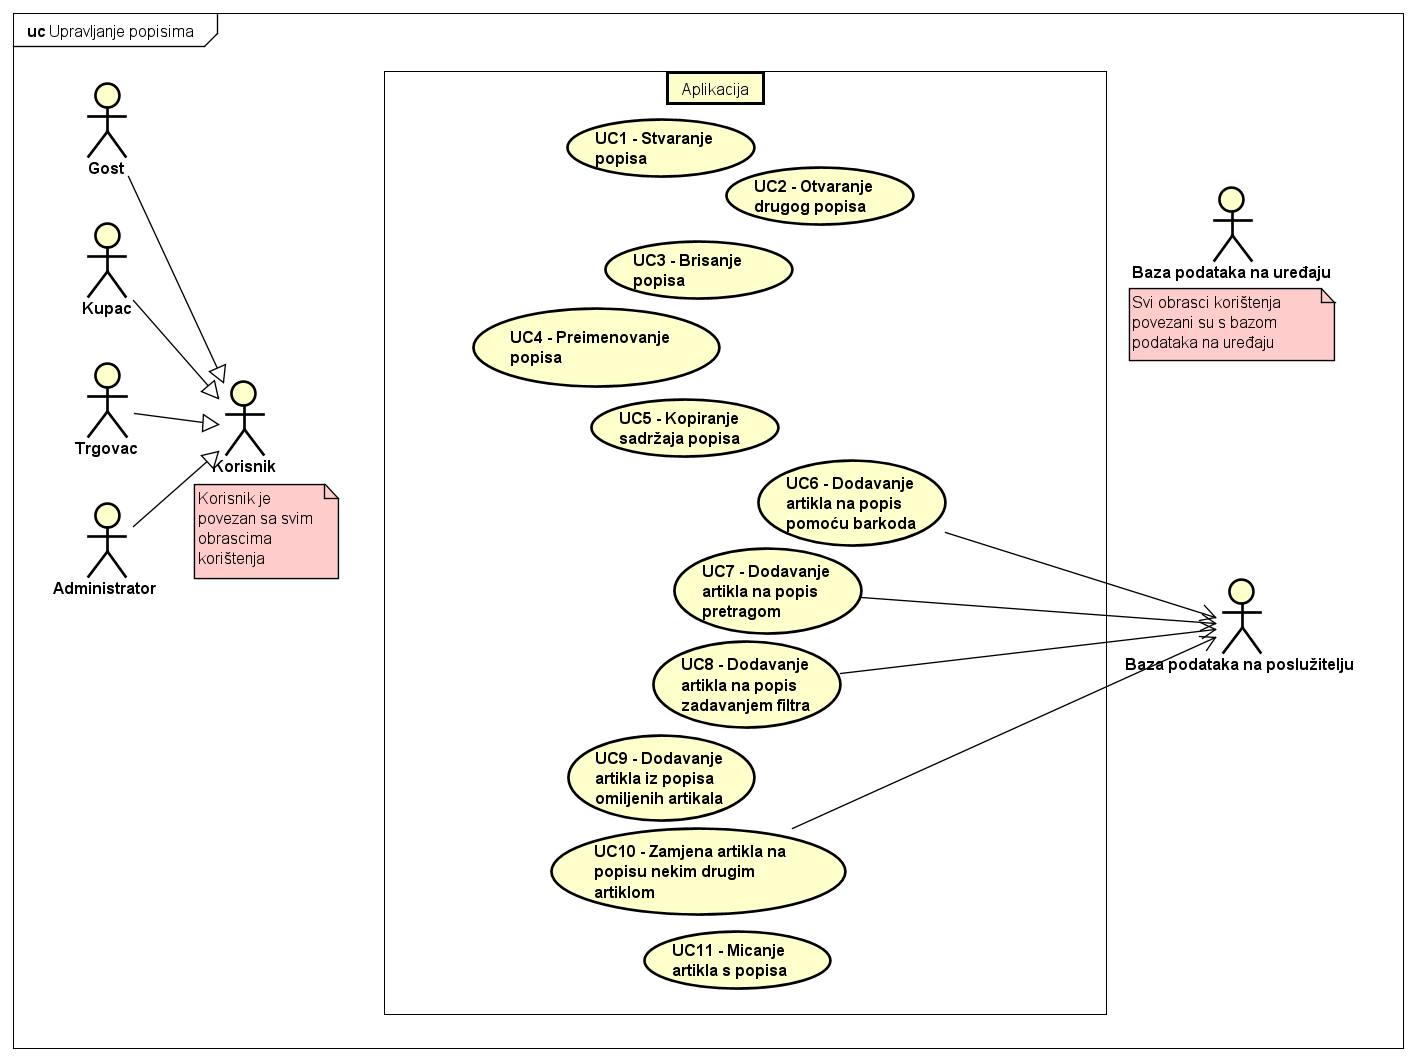
\includegraphics[width=.9\linewidth]{dijagrami/uc_upravljanje_popisima.png}
		            \label{fig:uc_upravljanje_popisima}
	                \end{center}
	            \end{figure}		
			    \begin{figure}[H]
			        \begin{center}
		            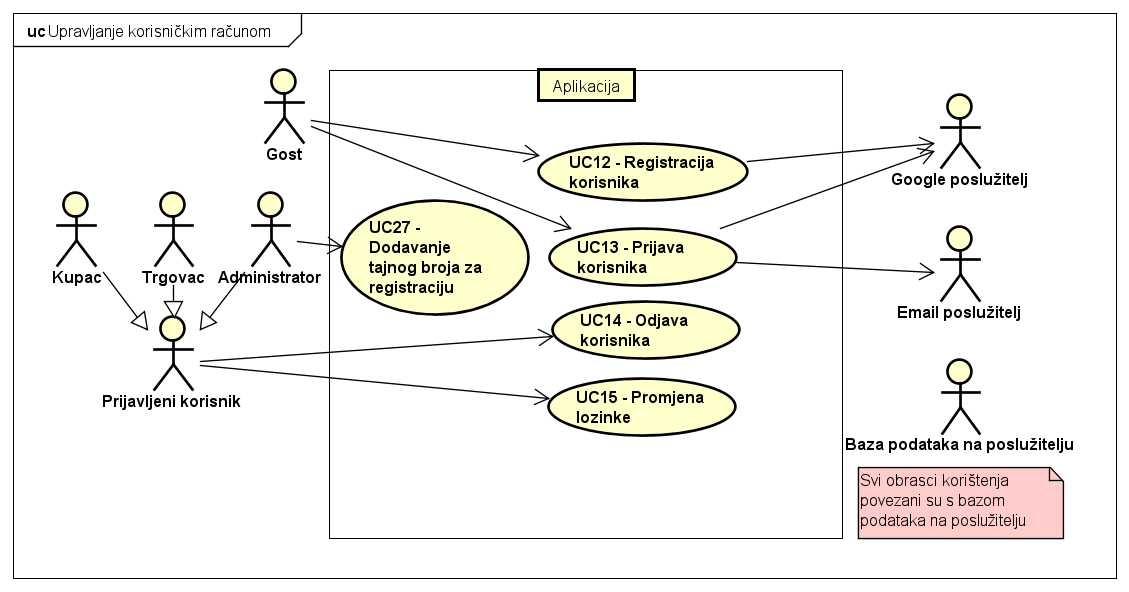
\includegraphics[width=.9\linewidth]{dijagrami/uc_kor_racun.png}
		            \label{fig:uc_kor_racun}
	                \end{center}
	            \end{figure}		
			    \begin{figure}[H]
			        \begin{center}
		            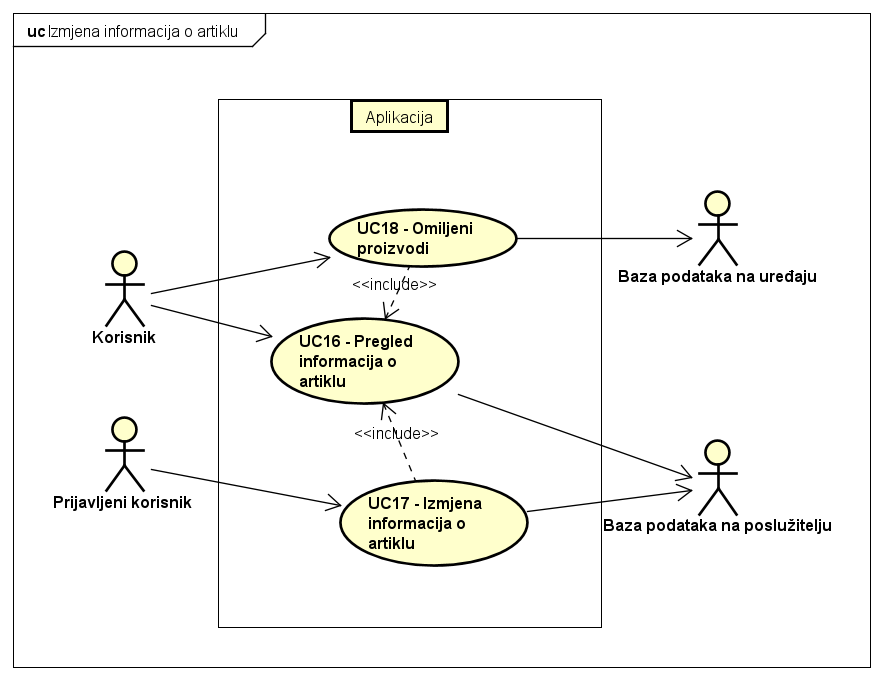
\includegraphics[width=.9\linewidth]{dijagrami/uc_info_artikl.png}
		            \label{fig:uc_info_artikl}
	                \end{center}
	            \end{figure}		
			    \begin{figure}[H]
			        \begin{center}
		            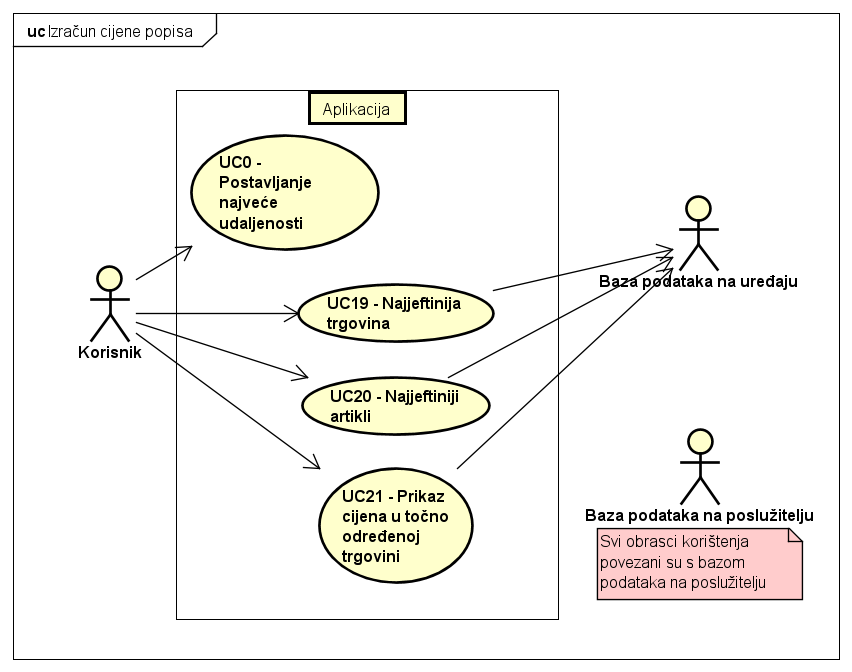
\includegraphics[width=.9\linewidth]{dijagrami/uc_cijena_popisa.png}
		            \label{fig:uc_cijena_popisa}
	                \end{center}
	            \end{figure}		
			    \begin{figure}[H]
			        \begin{center}
		            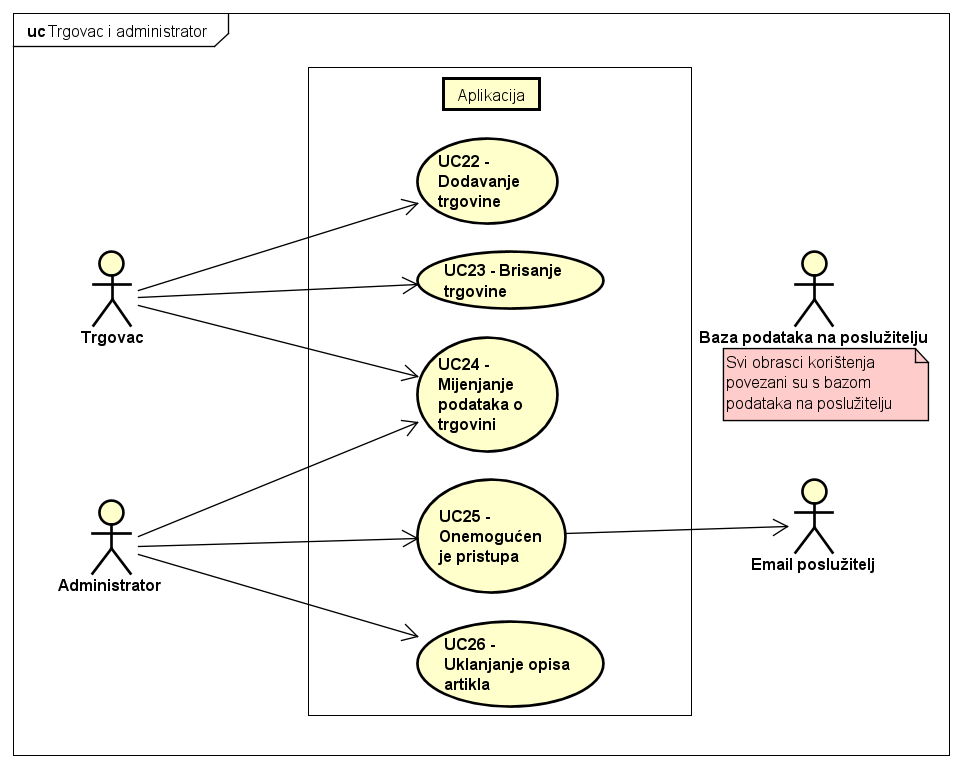
\includegraphics[width=.9\linewidth]{dijagrami/uc_trg_i_admin.png}
		            \label{fig:uc_trg_i_admin}
	                \end{center}
	            \end{figure}
	        
				\eject		
				
			\subsection{Sekvencijski dijagrami}
				
				\subsubsection{Obrazac uporabe UC7 - Dodavanje artikla na popis pretragom}
				    Korisnik pošalje traženo ime artikla. Poslužitelj iz baze podataka dohvaća barkodove i imena artikala sličnog imena. Prosljeđuje ih u listi korisniku. Ako lista nije prazna, korisnik odabire jedan od ponuđenih artikala i šalje poslužitelju njegov barkod i način izračuna cijene popisa, poslužitelj na temelju toga dohvati iz baze podataka informacije o artiklu i prosljeđuje ih cijenu korisniku. Korisnik ima sve potrebne informacije o stavci popisa i sprema ju u bazu podataka na uređaju.
	    \begin{figure}[H]
		    \centering
			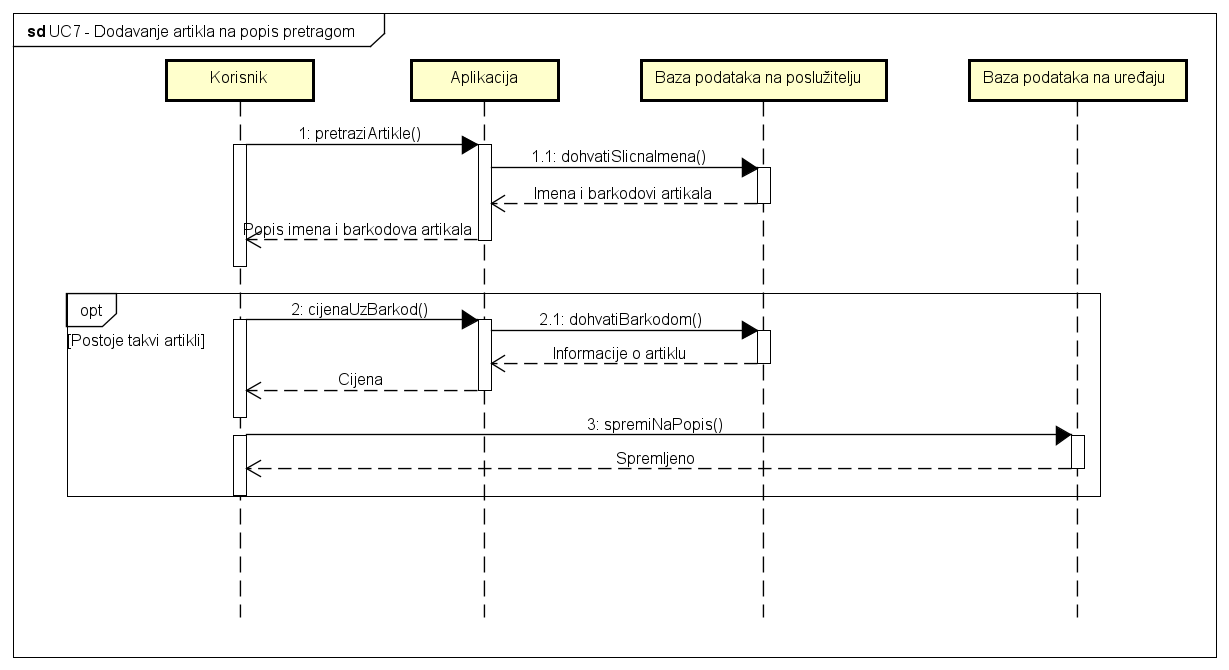
\includegraphics[width=0.9\linewidth]{dijagrami/sd_uc7.png}
			\caption{Sekvencijski dijagram za UC7}
			\label{fig:sd_uc7}
		\end{figure}
		
		
				\subsubsection{Obrazac uporabe UC13 - Prijava korisnika}
				    Ako se korisnik odlučio prijaviti Google računom, pošalje zahtjev za to poslužitelju koji provjerava njegove vjerodajnice zahtjevom prema Google poslužitelju. Ako su ispravne, u bazu podataka na poslužitelju sprema se token za korisnika i prijava je uspješna. Poslužitelj vraća rezultat prijave korisniku. \\
				    Ako se korisnik odlučio prijaviti email adresom i lozinkom, podatke za prijavu šalje na poslužitelj. Poslužitelj u bazi podataka provjerava jesu li ispravni. Ako jesu, poslužitelj sprema sjednički token u bazu podataka. na kraju poslužitelj vraća rezultat prijave korisniku. \\
				    Ako je korisnik odlučio zatražiti novu lozinku, šalje svoju email adresu poslužitelju. On provjerava u bazi podataka postoji li korisnik s tom email adresom. Ako postoji, generira privremenu lozinku, sprema ju u bazu podataka i šalje emailom korisniku preko email poslužitelja. Korisnik dobiva informaciju o tome je li lozinka poslana. \\
	    \begin{figure}[H]
		    \centering
			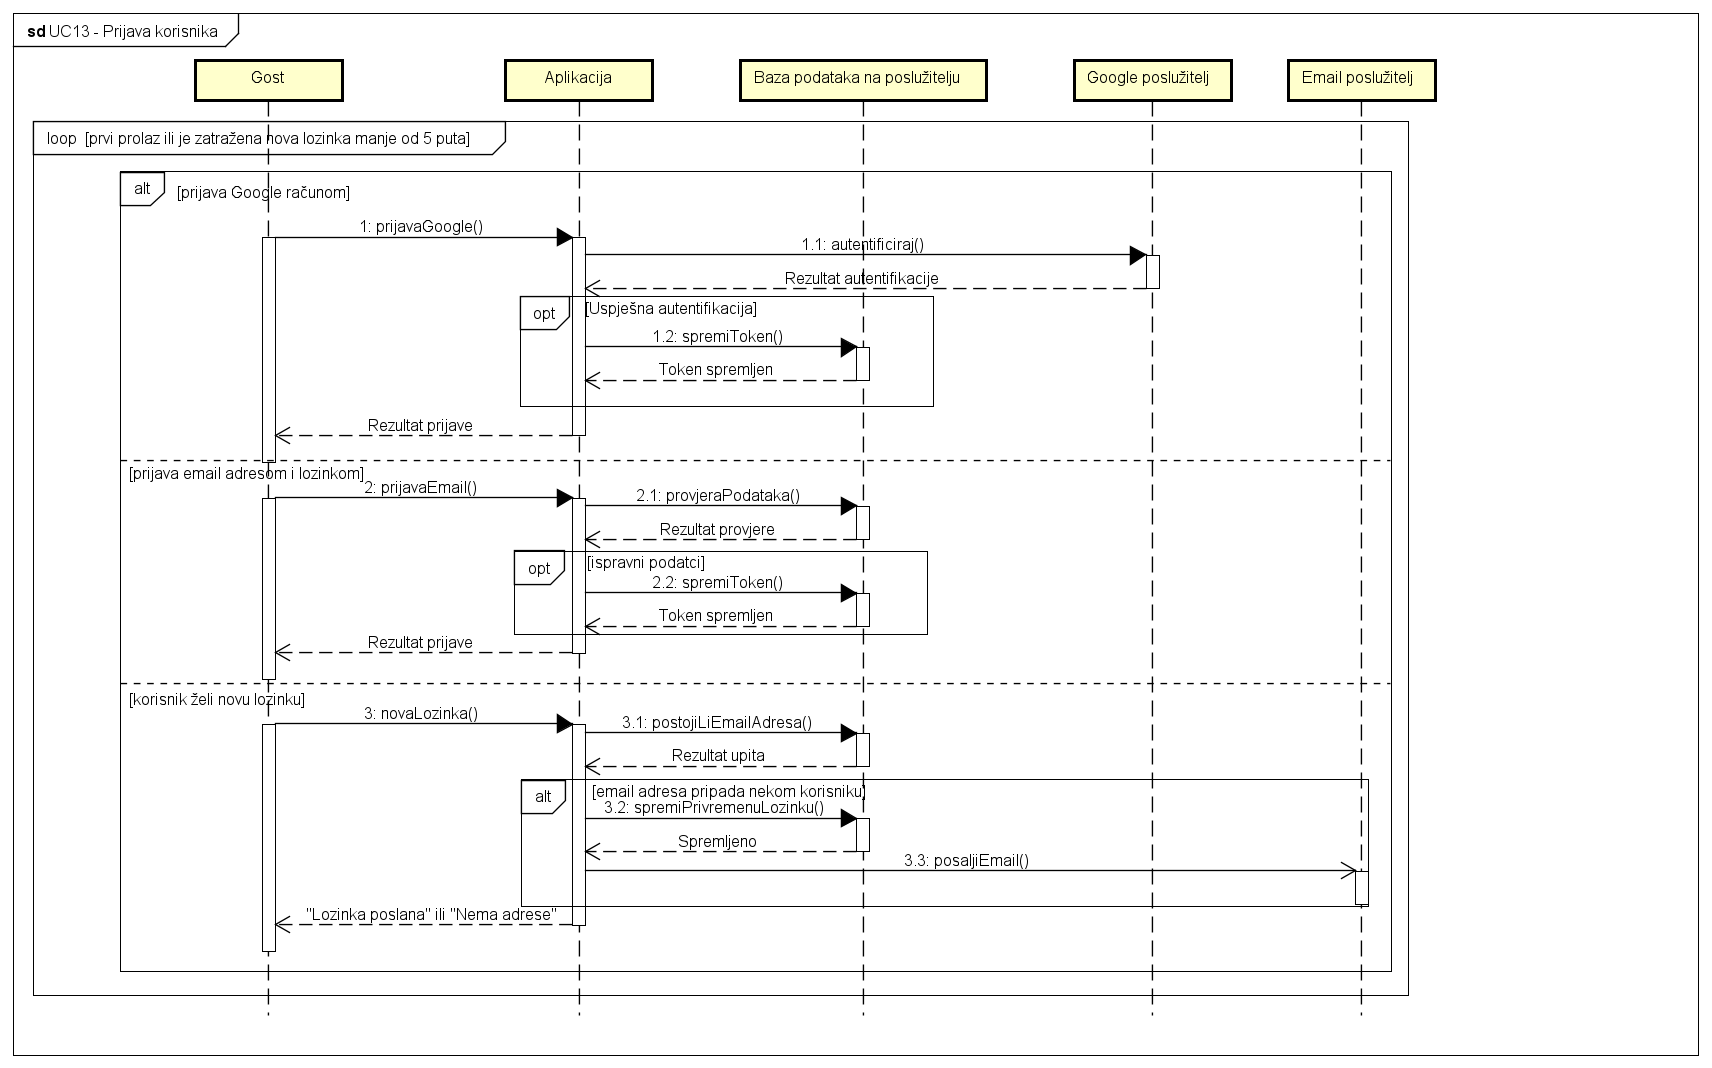
\includegraphics[width=1.0\linewidth]{dijagrami/sd_uc13.png}
			\caption{Sekvencijski dijagram za UC13}
			\label{fig:sd_uc13}
		\end{figure}
		
		
				\subsubsection{Obrazac uporabe UC17 - Izmjena informacija o artiklu}
				    Korisnik zatraži od poslužitelja informacije o artiklu. Korisnik dohvati informacije u bazi podataka i prosljeđuje ih korisniku. Ako korisnik zaključi da opis nije u redu, šalje zahtjev za smanjenjem broja glasova opisa. Poslužitelj ažurira broj glasova u bazi podataka i dohvati alternativne opise u bazi podataka koje zatim šalje korisniku. Ako se korisniku sviđa jedan od ponuđenih opisa, bira ga i tada se poslužitelju šalje zahtjev za povećanjem broja glasova opisa. Poslužitelj u bazi ažurira broj glasova i šalje korisniku povratnu informaciju. Ako se pak korisniku ne sviđa niti jedan od ponuđenih opisa, šalje svoj opis poslužitelju koji se sprema u bazu podataka i šalje zahtjev za smanjenjem broja glasova ponuđenih artikala. Poslužitelj ažurira broj glasova u bazi podataka i šalje povratnu informaciju korisniku.
	    \begin{figure}[H]
		    \centering
			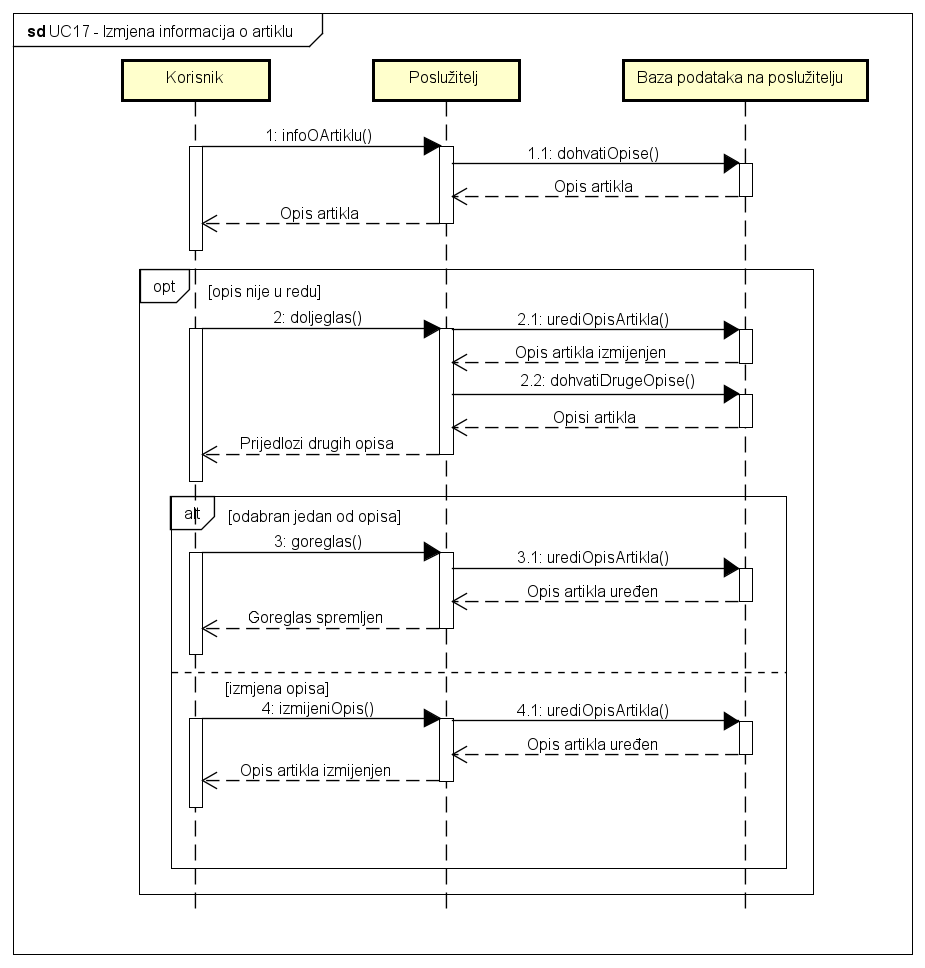
\includegraphics[width=1.0\linewidth]{dijagrami/sd_uc17.png}
			\caption{Sekvencijski dijagram za UC17}
			\label{fig:sd_uc17}
		\end{figure}
				\eject
	
		\section{Ostali zahtjevi}
        
        \begin{itemize}
            \item Aplikacija mora podržavati istovremeni rad 1000 korisnika
            \item Baza podataka mora odgovoriti na upit unutar pet sekundi
            \item Baza podataka mora podržavati unos 100 000 opisa artikala
            \item Baza podataka mora biti zaštićena od SQL injekcija
            \item Baza podataka mora biti otporna na napade duginom tablicom (rainbow table attack) dodavanjem predmetka lozinci
            \item Baza podataka mora lozinke raspršiti (hashing) pomoću funkcije SHA-256
            \item Pretpostavljena valuta sustava je HRK
            \item Korisničko sučelje mora podržavati hrvatski jezik i dijakritičke znakove
            \item Korisničko sučelje mora biti intuitivno
            \item Korisničko sučelje mora minimizirati broj koraka potrebnih da se učini neka akcija
            \item Neispravno korištenje korisničkog sučelja ne smije ugroziti rad sustava
            \item Aplikaciju mora biti moguće pokrenuti na Android uređajima inačice 5.0 naviše
        \end{itemize}
		 
			 %\textit{Nefunkcionalni zahtjevi i zahtjevi domene primjene dopunjuju funkcionalne zahtjeve. Oni opisuju \textbf{kako se sustav treba ponašati} i koja \textbf{ograničenja} treba poštivati (performanse, korisničko iskustvo, pouzdanost, standardi kvalitete, sigurnost...). Primjeri takvih zahtjeva u Vašem projektu mogu biti: podržani jezici korisničkog sučelja, vrijeme odziva, najveći mogući podržani broj korisnika, podržane web/mobilne platforme, razina zaštite (protokoli komunikacije, kriptiranje...)... Svaki takav zahtjev potrebno je navesti u jednoj ili dvije rečenice.}
			 
			 
			 
	

	\chapter{Arhitektura i dizajn sustava}

		Arhitektura je podijeljena na tri podsustava:
    \begin{packed_item}
        \item Mobilna aplikacija
        \item Poslužitelj
        \item Poslužitelj baze podataka
    \end{packed_item}
    
    Okviri i jezici koristimo izabrani su imajući na umu, između ostaloga, njihovu relativno dugotrajnu popularnost, što znači da osim male vjerojatnosti skore zastare postoji i veliki skup korisnika koji pružaju podršku, kao i problema koje su ti korisnici već riješili, a dostupni su na stranicama poput \url{stackoverflow.com}. Također su izvrsno dokumentirani. \\
    
	    \begin{figure}[H]
	        \begin{center}
            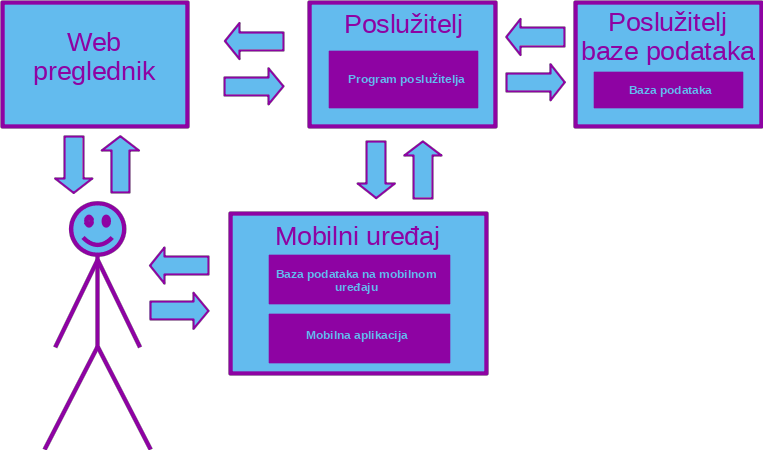
\includegraphics[width=1.0\linewidth]{slike/arh_skica.png}
            \caption{Skica arhitekture sustava}
            \label{fig:arh_skica}
            \end{center}
        \end{figure}
        
    \underbar{Aplikacija na mobilnom uređaju} napravljena je za sustav Android. Dio je frontend sloja, ali i u sklopu operativnog sustava komunicira s ugrađenom lokalnom bazom podataka (dakle nema zasebni poslužitelj). Preko protokola HTTP komunicira s poslužiteljem. Mobilna aplikacija napisana je u strojno podržanom (native) jeziku Androida - Java - koji je objektno orijentirani jezik što nam omogućuje podjelu u razrede koji su u paketima grupirani u međusobno povezane elemente, a pritom nam omogućuje i zadržavanje apstrakcije. Omogućuje nam i ponovnu iskoristivost jer bilo koji uređaj koji ima Java virtualni stroj može pokrenuti isti kôd. Android kao programski okvir omogućava veliku fleksibilnost (kroz razmještanje i imenovanje resursa prema dogovoru), poput automatske promjene jezika ovisno o korisničkim postavkama ili rezolucije slika ovisno o rezoluciji ekrana. \\
    \underbar{Kôd na poslužitelju} dio je backend sloja i napisan je u Pythonu 3 koji se, osim spomenutim prednostima objektno orijentirane paradigme, odlikuje i jednostavnošću kodiranja što značajno smanjuje vrijeme razvoja. Pogotovo uz backend okvir \textit{django} koji omogućava fleksibilnost ne koristeći "Convention over configuration" paradigmu, ali je i dalje jednostavan jer je pisan u Pythonu. Njegovo svojstvo "batteries included" smanjuje količinu posla razvojnom timu akcijama poput automatskog stvaranja sučelja za administratora kojemu se može pristupiti iz \underbar{web preglenika} korištenjem HTTP protokola te jednostavnog povezivanja s email poslužiteljem pomoću SMTP protokola. \\
    Koristimo stilističku varijaciju arhitekture zasnovane na događajima: MVC (\textit{Model, View, Controller}) obrazac. Kako mu i ime kaže, dijeli aplikaciju na model, pogled (View) i nadglednik (Controller). Time se omogućava odvajanje korisničkog sučelja (kroz pogled) od ostatka sustava. Za upravljanje zahtjevima korisnika služi nadglednik, a model opisuje strukturu i pravila vezane uz podatke. Podržava ga django. \\
  
	
		

		

				
		\section{Baze podataka}
		
		Za spremanje podataka koristimo, zbog njihove uvriježenosti i uglavnom velike sličnosti s našim poimanjem onoga što predstavljaju, relacijske baze podataka. One dijele informacije o objektima u atribute, a vrste objekata u tablice, tj. relacije. Takve baze podataka upravo postoje i optimirane su za učinkovito spremanje čitanje i izmjenu podatka, pa ih zato za to i koristimo. Konkretno, na poslužitelju smo se odlučili za PostgreSQL, a na Android uređaju imamo SQLite3. \\
		
		Slijede opisi tablica i njihovih veza. Imena atributa primarnog ključa deblje su otisnuta, a pozadinska boja ćelije u kojoj je ime stranog ključa promijenjena je u plavu.
			
			
		%--------------------------------------------------------------------------------
		

            \subsection{Opis tablica na uređaju}

                Tablica \underbar{omiljeni} sadrži šifre stavaka koje su označene kao omiljene. Tablica omiljeni je u \textit{Many-to-one} vezi s tablicom stavka (preko atributa sifStavka).
                \begin{longtabu} to \textwidth {|X[6, l]|X[6, l]|X[20, l]|}
                    
                    \hline \multicolumn{3}{|c|}{\textbf{omiljeni}}     \\[3pt] \hline
                    \endfirsthead
                    
                    \hline \multicolumn{3}{|c|}{\textbf{omiljeni}}     \\[3pt] \hline
                    \endhead
                    
                    \hline 
                    \endlastfoot

                    \cellcolor{LightBlue} \textbf{sifStavka} & INT & šifra stavke koja je označena kao omiljena \\ \hline
                    
                    
                    
                \end{longtabu}

                Tablica \underbar{popis} sadrži nazive popisa i njihove načine izračuna cijene. Tablica popis je u \textit{One-to-many} vezi s tablicom stavka (preko atributa sifPopis).
                \begin{longtabu} to \textwidth {|X[6, l]|X[6, l]|X[20, l]|}
                    
                    \hline \multicolumn{3}{|c|}{\textbf{popis}}     \\[3pt] \hline
                    \endfirsthead
                    
                    \hline \multicolumn{3}{|c|}{\textbf{popis}}     \\[3pt] \hline
                    \endhead
                    
                    \hline 
                    \endlastfoot

                    \textbf{sifPopis} & INT & šifra popisa \\ \hline
                    nazivPopis & NCHAR VARYING & naziv popisa \\ \hline
                    izrCijene & BIT & način izračuna cijene \\ \hline
                    sifTrgovina & INT & šifra trgovine vezane uz popis (ako je primjenjivo) \\ \hline
                    
                    
                    
                \end{longtabu}

                Tablica \underbar{stavka} sadrži stavke na popisu. Tablica stavka je u \textit{One-to-many} vezi s tablicom omiljeni (preko atributa sifStavka). Tablica stavka je u \textit{Many-to-one} vezi s tablicom popis (preko atributa sifPopis).
                \begin{longtabu} to \textwidth {|X[6, l]|X[6, l]|X[20, l]|}
                    
                    \hline \multicolumn{3}{|c|}{\textbf{stavka}}     \\[3pt] \hline
                    \endfirsthead
                    
                    \hline \multicolumn{3}{|c|}{\textbf{stavka}}     \\[3pt] \hline
                    \endhead
                    
                    \hline 
                    \endlastfoot

                    \textbf{sifStavka} & INT & šifra stavke \\ \hline
                    \cellcolor{LightBlue} sifPopis & INT & šifra popisa na kojem je stavka \\ \hline
                    barkod & DECIMAL & barkod artikla \\ \hline
                    cijena & DECIMAL & cijena artikla \\ \hline
                    filtarFunkcija & VARCHAR & sadrži sažeto napisane filtar funkcije koje se primjenjuju \\ \hline
                    uKosarici & BIT & oznaka je li stavka dodana u košaricu \\ \hline
                    kolicina & DECIMAL & količina artikla u intervalu [0,000 - 999,999] \\ \hline
                    naziv & NCHAR VARYING & naziv artikla \\ \hline
                    sifTrgovina & INT & šifra trgovine vezane uz cijenu \\ \hline
                    
                    
                    
                \end{longtabu}



            \subsection{Opis tablica na posluzitelju}

                Tablica \underbar{artikl} sadrži popis svih barkodova artikala. Tablica artikl je u \textit{One-to-many} vezi s tablicom opisArtikla (preko atributa barkod) i tablicom artiklUTrgovini (preko atributa barkod).
                \begin{longtabu} to \textwidth {|X[6, l]|X[6, l]|X[20, l]|}
                    
                    \hline \multicolumn{3}{|c|}{\textbf{artikl}}     \\[3pt] \hline
                    \endfirsthead
                    
                    \hline \multicolumn{3}{|c|}{\textbf{artikl}}     \\[3pt] \hline
                    \endhead
                    
                    \hline 
                    \endlastfoot

                    \textbf{barkod} & DECIMAL & barkod artikla \\ \hline
                    
                    
                    
                \end{longtabu}

                Tablica \underbar{artiklUTrgovini} sadrži popis artikala u trgovini. Tablica artiklUTrgovini je u \textit{Many-to-one} vezi s tablicom artikl (preko atributa barkod), tablicom trgovina (preko atributa sifTrgovina) i tablicom opisArtikla (preko atributa barkod i email).
                \begin{longtabu} to \textwidth {|X[6, l]|X[6, l]|X[20, l]|}
                    
                    \hline \multicolumn{3}{|c|}{\textbf{artiklUTrgovini}}     \\[3pt] \hline
                    \endfirsthead
                    
                    \hline \multicolumn{3}{|c|}{\textbf{artiklUTrgovini}}     \\[3pt] \hline
                    \endhead
                    
                    \hline 
                    \endlastfoot

                    \cellcolor{LightBlue} \textbf{barkod} & DECIMAL & barkod artikla \\ \hline
                    \cellcolor{LightBlue} \textbf{sifTrgovina} & CHAR & šifra trgovine \\ \hline
                    \cellcolor{LightBlue} email & VARCHAR & email vezan uz željeni opis \\ \hline
                    cijena & DECIMAL & cijena artikla u trgovini \\ \hline
                    popust & FLOAT & popust na cijenu artikla u trgovini \\ \hline
                    dostupnost & BIT & ima li artikla u trgovini \\ \hline
                    
                    
                    
                \end{longtabu}

                Tablica \underbar{kategorija} sadrži popis kategorija artikala. Tablica kategorija je u \textit{One-to-many} vezi s tablicom potkategorija (preko atributa sifKategorija).
                \begin{longtabu} to \textwidth {|X[6, l]|X[6, l]|X[20, l]|}
                    
                    \hline \multicolumn{3}{|c|}{\textbf{kategorija}}     \\[3pt] \hline
                    \endfirsthead
                    
                    \hline \multicolumn{3}{|c|}{\textbf{kategorija}}     \\[3pt] \hline
                    \endhead
                    
                    \hline 
                    \endlastfoot

                    \textbf{sifKategorija} & INT & šifra kategorije artikla \\ \hline
                    nazivKategorija & NCHAR VARYING & naziv kategorije artikla \\ \hline
                    
                    
                    
                \end{longtabu}

                Tablica \underbar{korisnik} sadrži informacije o prijavljenim korisnicima aplikacije. Tablica korisnik je u \textit{One-to-many} vezi s tablicom onemoguceniRacun (preko atributa email), tablicom opisArtikla (preko atributa email), tablicom privremenaLozinka (preko atributa email) i tablicom trgovina (preko atributa email). Tablica korisnik je u \textit{Many-to-one} vezi s tablicom uloga (preko atributa sifUloga).
                \begin{longtabu} to \textwidth {|X[6, l]|X[6, l]|X[20, l]|}
                    
                    \hline \multicolumn{3}{|c|}{\textbf{korisnik}}     \\[3pt] \hline
                    \endfirsthead
                    
                    \hline \multicolumn{3}{|c|}{\textbf{korisnik}}     \\[3pt] \hline
                    \endhead
                    
                    \hline 
                    \endlastfoot

                    \textbf{email} & VARCHAR & email korisnika \\ \hline
                    \cellcolor{LightBlue} sifUloga & INT & šifra uloge korisnika \\ \hline
                    lozinka & VARCHAR & hash lozinke korisnika (SHA 256) \\ \hline
                    token & CHAR & token sjednice korisnika \\ \hline
                    
                    
                    
                \end{longtabu}

                Tablica \underbar{onemoguceniRacun} sadrži popis onemogućenih računa. Tablica onemoguceniRacun je u \textit{Many-to-one} vezi s tablicom korisnik (preko atributa adminEmail).
                \begin{longtabu} to \textwidth {|X[6, l]|X[6, l]|X[20, l]|}
                    
                    \hline \multicolumn{3}{|c|}{\textbf{onemoguceniRacun}}     \\[3pt] \hline
                    \endfirsthead
                    
                    \hline \multicolumn{3}{|c|}{\textbf{onemoguceniRacun}}     \\[3pt] \hline
                    \endhead
                    
                    \hline 
                    \endlastfoot

                    \cellcolor{LightBlue} \textbf{onemoguceni} & VARCHAR & email osobe kojoj je onemogućen pristup \\ \hline
                    \cellcolor{LightBlue} \textbf{adminEmail} & VARCHAR & email admina koji je onemogućio osobi pristup \\ \hline
                    datum & DATE & datum onemogućenja \\ \hline
                    
                    
                    
                \end{longtabu}

                Tablica \underbar{opisArtikla} sadrži opis i informacije vezane uz artikl zadan barkodom koje je napisao neki prijavljeni korisnik. Tablica opisArtikla je u \textit{One-to-many} vezi s tablicom artiklUTrgovini (preko atributa barkod i email). Tablica opisArtikla je u \textit{Many-to-one} vezi s tablicom artikl (preko atributa barkod), tablicom korisnik (preko atributa email), tablicom vrsta (preko atributa sifKategorija, sifPotkategorija i sifVrsta) i tablicom zemlja (preko atributa sifZemlja).
                \begin{longtabu} to \textwidth {|X[6, l]|X[6, l]|X[20, l]|}
                    
                    \hline \multicolumn{3}{|c|}{\textbf{opisArtikla}}     \\[3pt] \hline
                    \endfirsthead
                    
                    \hline \multicolumn{3}{|c|}{\textbf{opisArtikla}}     \\[3pt] \hline
                    \endhead
                    
                    \hline 
                    \endlastfoot

                    \cellcolor{LightBlue} \textbf{barkod} & DECIMAL & barkod artikla \\ \hline
                    \cellcolor{LightBlue} \textbf{email} & VARCHAR & email osobe koja je napisala opis \\ \hline
                    \cellcolor{LightBlue} sifKategorija & INT & šifra kategorije artikla \\ \hline
                    \cellcolor{LightBlue} sifPotkategorija & INT & šifra potkategorije artikla \\ \hline
                    \cellcolor{LightBlue} sifVrsta & INT & šifra vrste artikla \\ \hline
                    \cellcolor{LightBlue} sifZemlja & CHAR & šifra zemlje podrijetla \\ \hline
                    kratkiOpis & NCHAR VARYING & kratki opis artikla (do 255 znakova) \\ \hline
                    nazivArtikla & NCHAR VARYING & naziv artikla (do 32 znaka) \\ \hline
                    brojGlasova & INT & broj glasova o opisu artikla (goreglasovi - doljeglasovi) \\ \hline
                    masa & INT & masa artikla \\ \hline
                    
                    
                    
                \end{longtabu}

                Tablica \underbar{potkategorija} sadrži popis potkategorija artikala. Tablica potkategorija je u \textit{One-to-many} vezi s tablicom vrsta (preko atributa sifKategorija i sifPotkategorija). Tablica potkategorija je u \textit{Many-to-one} vezi s tablicom kategorija (preko atributa sifKategorija).
                \begin{longtabu} to \textwidth {|X[6, l]|X[6, l]|X[20, l]|}
                    
                    \hline \multicolumn{3}{|c|}{\textbf{potkategorija}}     \\[3pt] \hline
                    \endfirsthead
                    
                    \hline \multicolumn{3}{|c|}{\textbf{potkategorija}}     \\[3pt] \hline
                    \endhead
                    
                    \hline 
                    \endlastfoot

                    \cellcolor{LightBlue} \textbf{sifKategorija} & INT & šifra kategorije kojoj potkategorija artikla pripada \\ \hline
                    \textbf{sifPotkategorija} & INT & šifra podkategorije artikla \\ \hline
                    nazivPotkategorija & NCHAR VARYING & naziv potkategorije artikla \\ \hline
                    
                    
                    
                \end{longtabu}

                Tablica \underbar{privremenaLozinka} sadrži privremene lozinke poslane na email korisnika. Tablica privremenaLozinka je u \textit{Many-to-one} vezi s tablicom korisnik (preko atributa email).
                \begin{longtabu} to \textwidth {|X[6, l]|X[6, l]|X[20, l]|}
                    
                    \hline \multicolumn{3}{|c|}{\textbf{privremenaLozinka}}     \\[3pt] \hline
                    \endfirsthead
                    
                    \hline \multicolumn{3}{|c|}{\textbf{privremenaLozinka}}     \\[3pt] \hline
                    \endhead
                    
                    \hline 
                    \endlastfoot

                    \cellcolor{LightBlue} \textbf{email} & VARCHAR & email korisnika koji je zatrazio promjenu \\ \hline
                    lozinka & CHAR & hash privremene lozinke \\ \hline
                    istice & DATE & datum isteka lozinke \\ \hline
                    
                    
                    
                \end{longtabu}

                Tablica \underbar{tajniBroj} sadrži popis tajnih brojeva za registraciju. Tablica tajniBroj je u \textit{Many-to-one} vezi s tablicom uloga (preko atributa sifUloga).
                \begin{longtabu} to \textwidth {|X[6, l]|X[6, l]|X[20, l]|}
                    
                    \hline \multicolumn{3}{|c|}{\textbf{tajniBroj}}     \\[3pt] \hline
                    \endfirsthead
                    
                    \hline \multicolumn{3}{|c|}{\textbf{tajniBroj}}     \\[3pt] \hline
                    \endhead
                    
                    \hline 
                    \endlastfoot

                    \textbf{broj} & INT & tajni broj \\ \hline
                    \cellcolor{LightBlue} sifUloga & INT & šifra uloge koju će korisnik poprimiti \\ \hline
                    idKorisnika & INT & neki identifikator osobe koja će iskoristiti tajni broj \\ \hline
                    
                    
                    
                \end{longtabu}

                Tablica \underbar{trgovina} sadrži informacije o trgovinama. Tablica trgovina je u \textit{One-to-many} vezi s tablicom artiklUTrgovini (preko atributa sifTrgovina). Tablica trgovina je u \textit{Many-to-one} vezi s tablicom korisnik (preko atributa email).
                \begin{longtabu} to \textwidth {|X[6, l]|X[6, l]|X[20, l]|}
                    
                    \hline \multicolumn{3}{|c|}{\textbf{trgovina}}     \\[3pt] \hline
                    \endfirsthead
                    
                    \hline \multicolumn{3}{|c|}{\textbf{trgovina}}     \\[3pt] \hline
                    \endhead
                    
                    \hline 
                    \endlastfoot

                    \textbf{sifTrgovina} & CHAR & šiftra trgovine \\ \hline
                    \cellcolor{LightBlue} email & VARCHAR & email vlasnika trgovine \\ \hline
                    lat & DECIMAL & geografska širina trgovine \\ \hline
                    lon & DECIMAL & geografska dužina trgovine \\ \hline
                    nazivTrgovina & NCHAR & naziv trgovine \\ \hline
                    adresa & VARCHAR & adresa trgovine \\ \hline
                    radnoVrijemePoc & TIME & početak radnog vremena trgovine \\ \hline
                    radnoVrijemeKraj & TIME & kraj radnog vremena \\ \hline
                    
                    
                    
                \end{longtabu}

                Tablica \underbar{uloga} sadrži popis uloga koje prijavljeni korisnik može poprimiti (administrator, trgovac ili kupac). Tablica uloga je u \textit{One-to-many} vezi s tablicom korisnik (preko atributa sifUloga) i tablicom tajniBroj (preko atributa sifUloga).
                \begin{longtabu} to \textwidth {|X[6, l]|X[6, l]|X[20, l]|}
                    
                    \hline \multicolumn{3}{|c|}{\textbf{uloga}}     \\[3pt] \hline
                    \endfirsthead
                    
                    \hline \multicolumn{3}{|c|}{\textbf{uloga}}     \\[3pt] \hline
                    \endhead
                    
                    \hline 
                    \endlastfoot

                    \textbf{sifUloga} & INT & šifra uloge korisnika \\ \hline
                    nazUloga & VARCHAR & naziv uloge prijavljenog korisnika \\ \hline
                    
                    
                    
                \end{longtabu}

                Tablica \underbar{vrsta} sadrži popis vrsta artikala. Tablica vrsta je u \textit{One-to-many} vezi s tablicom opisArtikla (preko atributa sifKategorija, sifPotkategorija i sifVrsta). Tablica vrsta je u \textit{Many-to-one} vezi s tablicom potkategorija (preko atributa sifKategorija i sifPotkategorija).
                \begin{longtabu} to \textwidth {|X[6, l]|X[6, l]|X[20, l]|}
                    
                    \hline \multicolumn{3}{|c|}{\textbf{vrsta}}     \\[3pt] \hline
                    \endfirsthead
                    
                    \hline \multicolumn{3}{|c|}{\textbf{vrsta}}     \\[3pt] \hline
                    \endhead
                    
                    \hline 
                    \endlastfoot

                    \cellcolor{LightBlue} \textbf{sifKategorija} & INT & šifra kategorije kojoj vrsta artikla pripada \\ \hline
                    \cellcolor{LightBlue} \textbf{sifPotkategorija} & INT & šifra potkategorije kojoj vrsta artikla pripada \\ \hline
                    \textbf{sifVrsta} & INT & šifra vrste \\ \hline
                    nazivVrsta & NCHAR VARYING & naziv vrste artikla \\ \hline
                    
                    
                    
                \end{longtabu}

                Tablica \underbar{zemlja} sadrži popis zemalja koje korisnik može odabrati kao zemlju podrijetla. Tablica zemlja je u \textit{One-to-many} vezi s tablicom opisArtikla (preko atributa sifZemlja).
                \begin{longtabu} to \textwidth {|X[6, l]|X[6, l]|X[20, l]|}
                    
                    \hline \multicolumn{3}{|c|}{\textbf{zemlja}}     \\[3pt] \hline
                    \endfirsthead
                    
                    \hline \multicolumn{3}{|c|}{\textbf{zemlja}}     \\[3pt] \hline
                    \endhead
                    
                    \hline 
                    \endlastfoot

                    \textbf{sifZemlja} & CHAR & šifra zemlje podrijetla \\ \hline
                    nazivZemlja & NCHAR VARYING & naziv zemlje podrijetla \\ \hline
                    
                    
                    
                \end{longtabu}

		%------------------------------------------------------------------------------
			\subsection{Dijagrami baze podataka}
		\begin{figure}[H]
		    \centering
			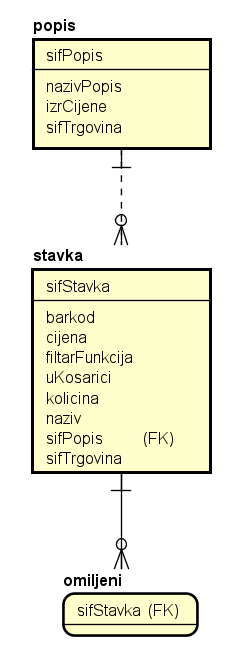
\includegraphics[scale=0.4]{dijagrami/db_uredaj.png}
			\caption{Baza podataka na uređaju}
			\label{fig:db_uredaj}
		\end{figure}
		
		\begin{figure}[H]
		    \centering
			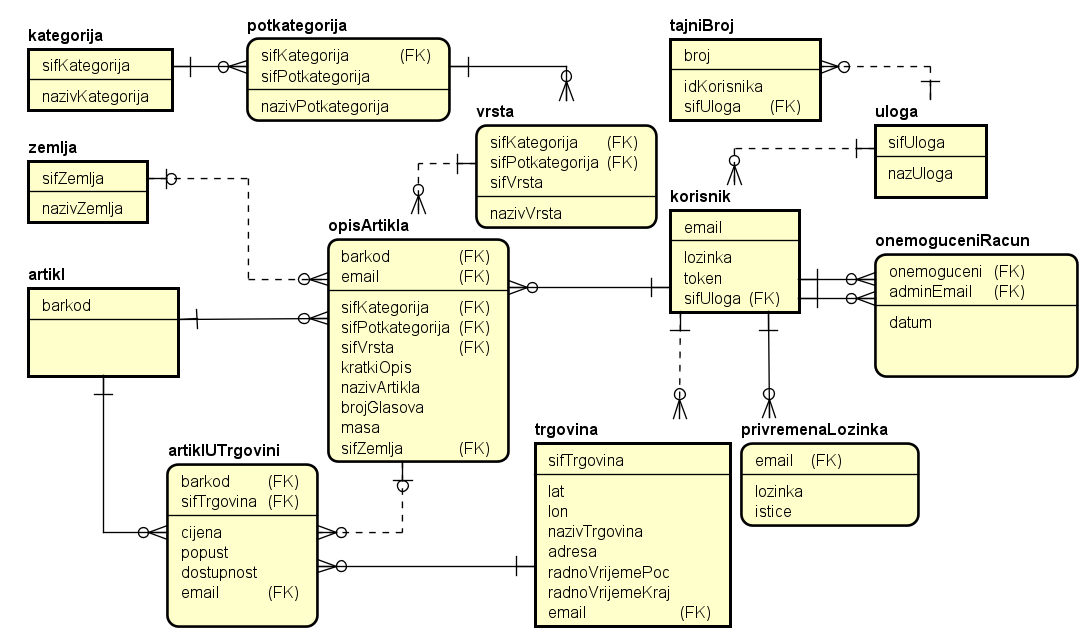
\includegraphics[width=.9\linewidth]{dijagrami/db_posluzitelj.png}
			\caption{Baza podataka na poslužitelju}
			\label{fig:db_posluzitelj}
		\end{figure}
			
			\eject
			
			
		\section{Dijagrami razreda}
		
		Dijagram razreda na uređaju sadrži klase koje nisu dio generične funkcionalnosti, ali su ubačene radi preglednosti. To su List, Listitem, RoomDB, Favourites i About
		
		\begin{figure}[H]
		    \centering
			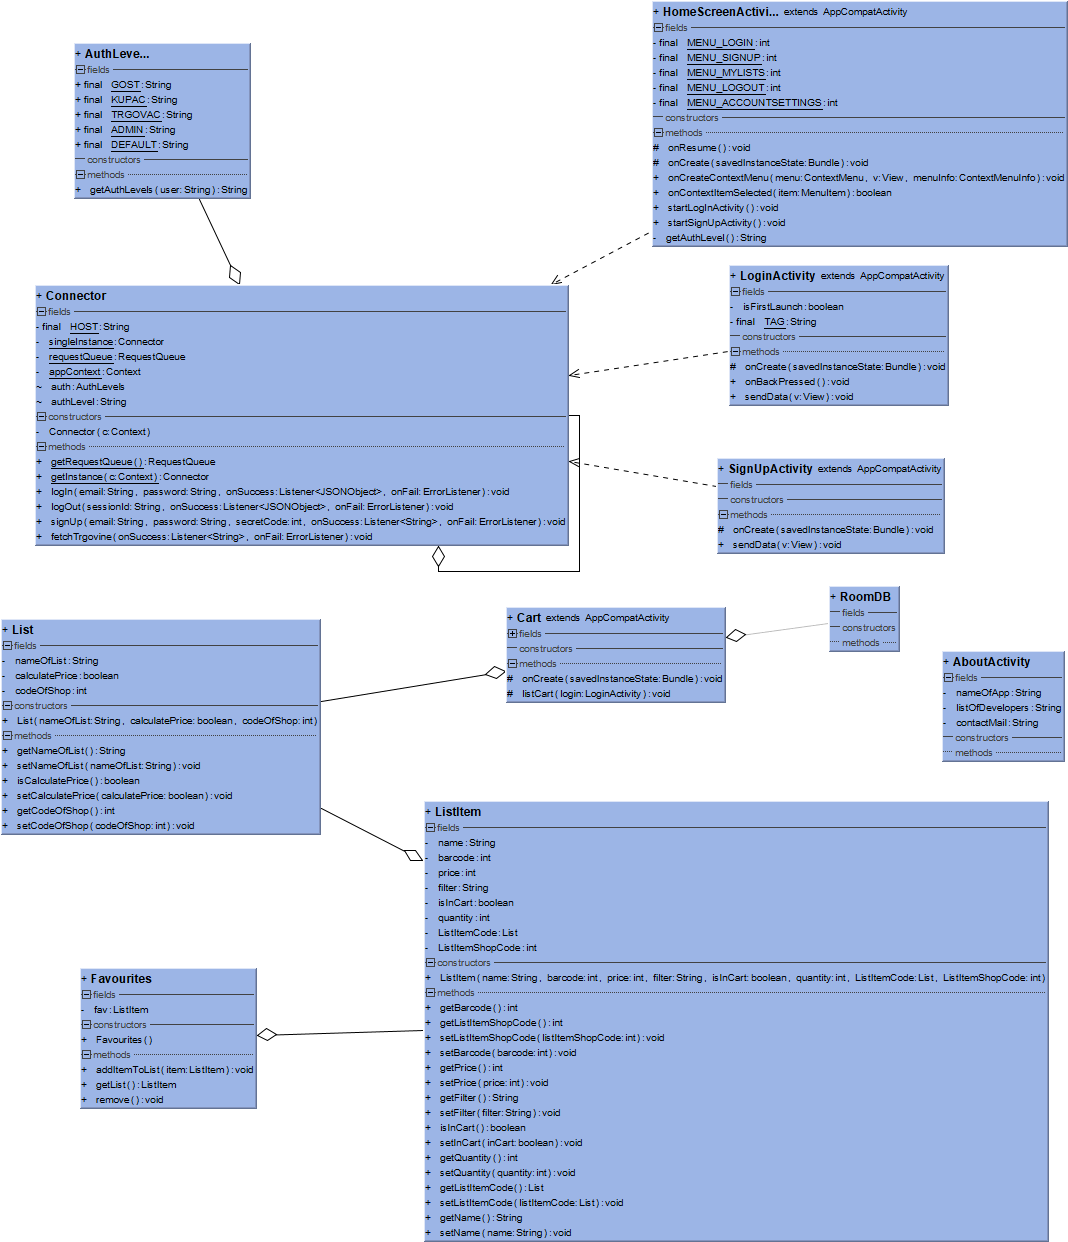
\includegraphics[scale=0.4]{dijagrami/class_uredaj.png}
			\caption{Dijagram razreda na uređaju}
			\label{fig:class_uredaj}
		\end{figure}
		
	
		\begin{figure}[H]
			\centering
			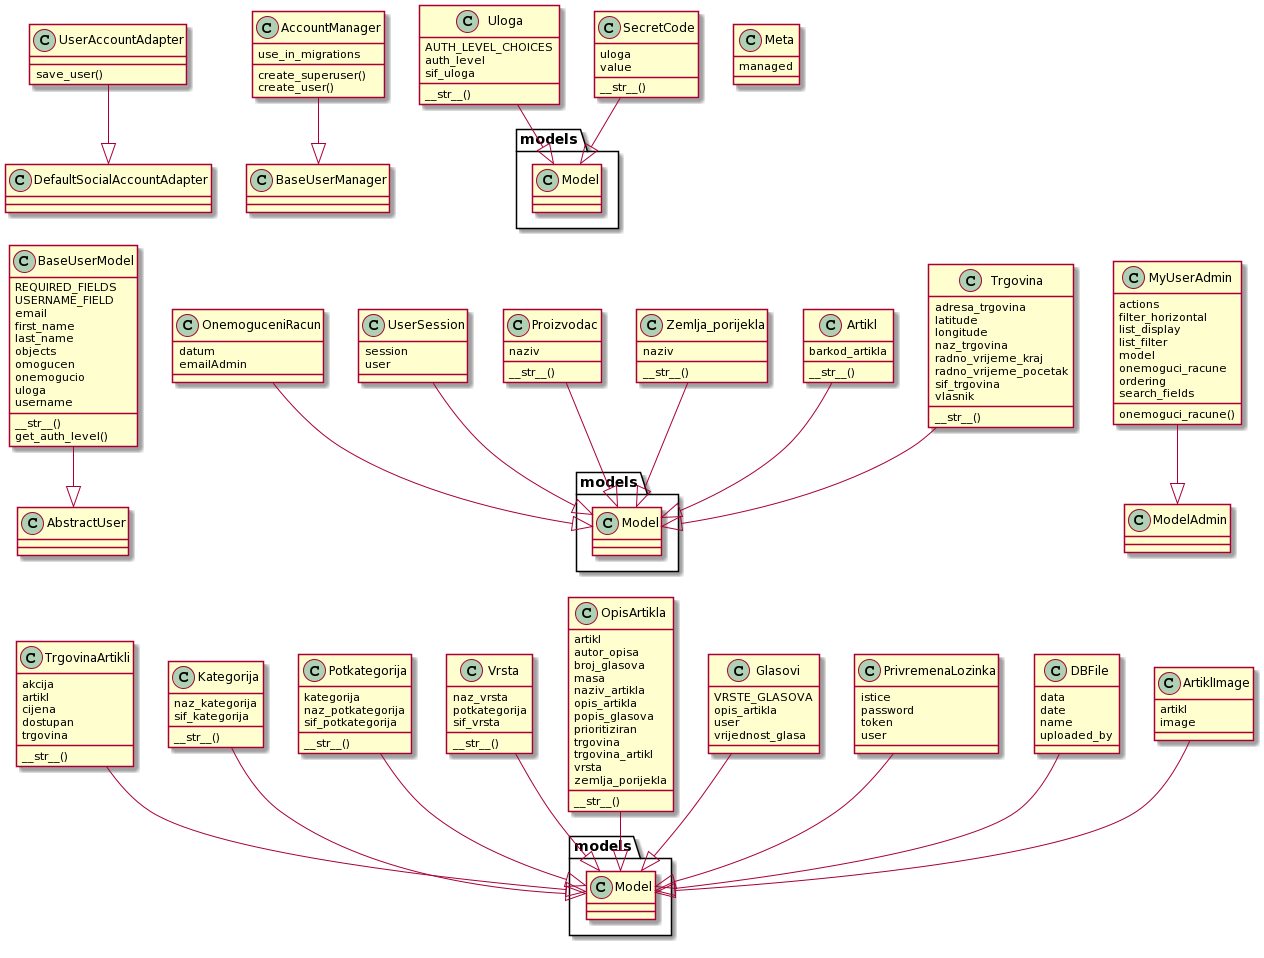
\includegraphics[width=1.0\linewidth]{dijagrami/class.png}
			\caption{Dijagram razreda na poslužitelju}
			\label{fig:class}
		\end{figure}
	
		\section{Dijagram stanja}
			Priložena su dva dijagrama stanja. Jedan prikazuje web stranicu na kojoj korisnik nije ulogiran, a drugi dijagram stanja prikazuje web stranicu na kojoj je ulogiran trgovac.
			
			Dijagram stanja koji opisuje web stranicu na kojoj korisnik nije ulogiran nudi nekoliko opcija: prijava, registracija kao kupac i registracija kao trgovac. Registrirati se kao može bilo tko samo jednom s istom email adresom. Za registraciju kao kupac nisu potrebni nikakvi preduvjeti, dok je za registraciju kao trgovac potreban odgovarajući kod.
			
			
			
			\begin{figure}[H]
				\centering
				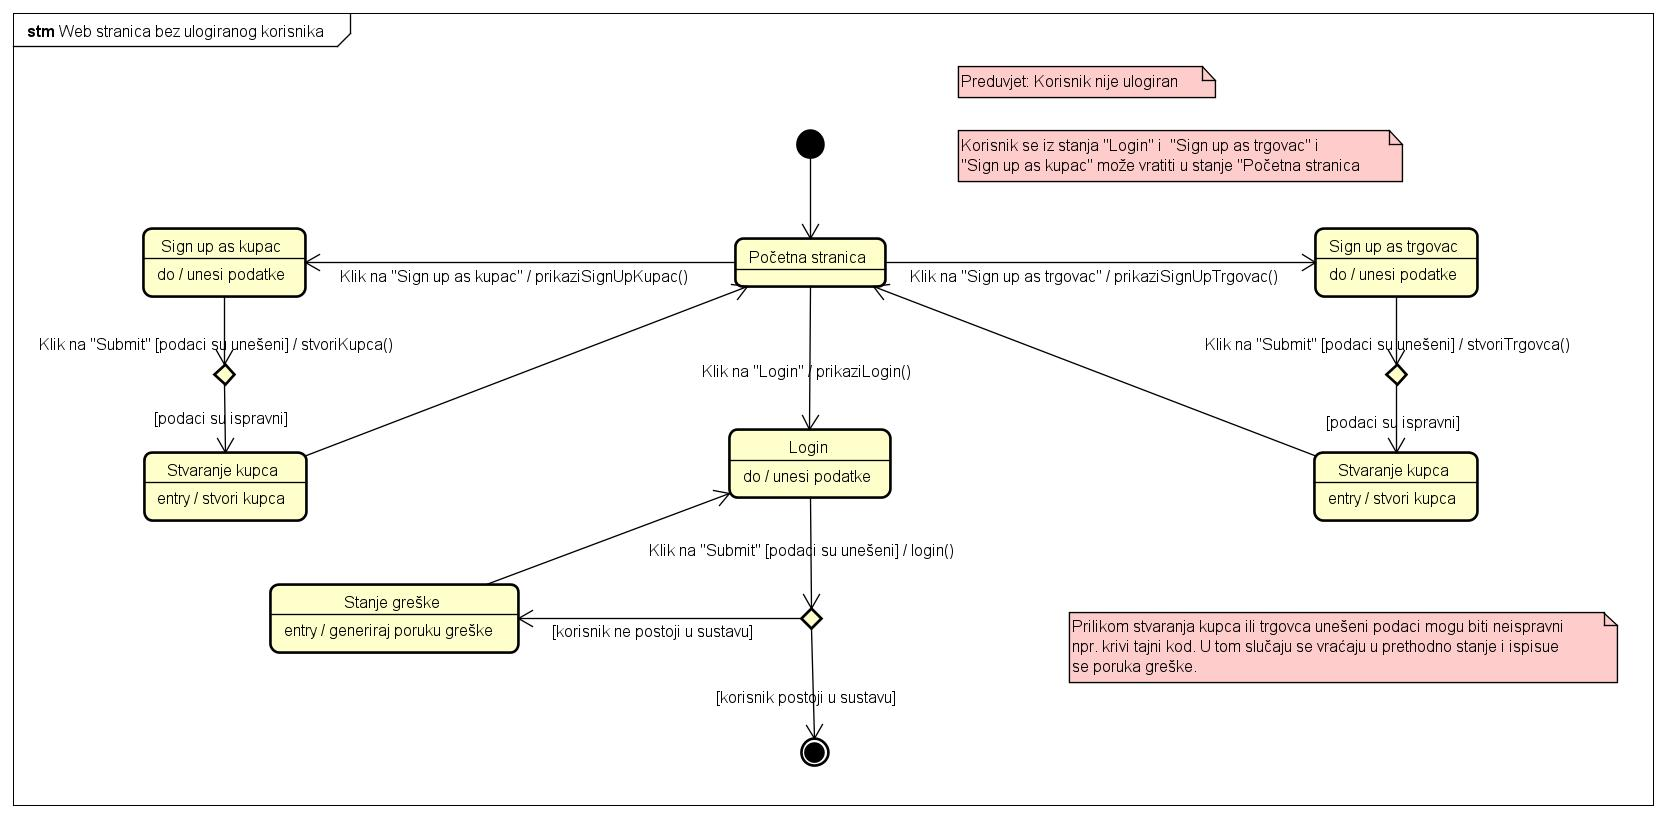
\includegraphics[width=1.0\linewidth]{dijagrami/web-neulogiran.jpg}
				\caption{Dijagram stanja web stranice za neulogiranog korisnika}
				\label{fig:state-web-neulogiran}
			\end{figure}
		
			Sljedeći dijagram stanja opisuje web stranicu na kojoj je ulogiran trgovac. On ima već nabrojane opcije kao što su pregled trgovina, dodavanje trgovine, pregled proizvoda u trgovini, brisanje proizvoda u trgovini itd. Preduvjet za svaku akciju brisanja je naravno da proizvod koji se želi obrisati postoji. Također, što se tiče pregleda trgovine, trgovac može pregledati samo onu trgovinu za koju je on zadužen.
		
			\begin{figure}[H]
				\centering
				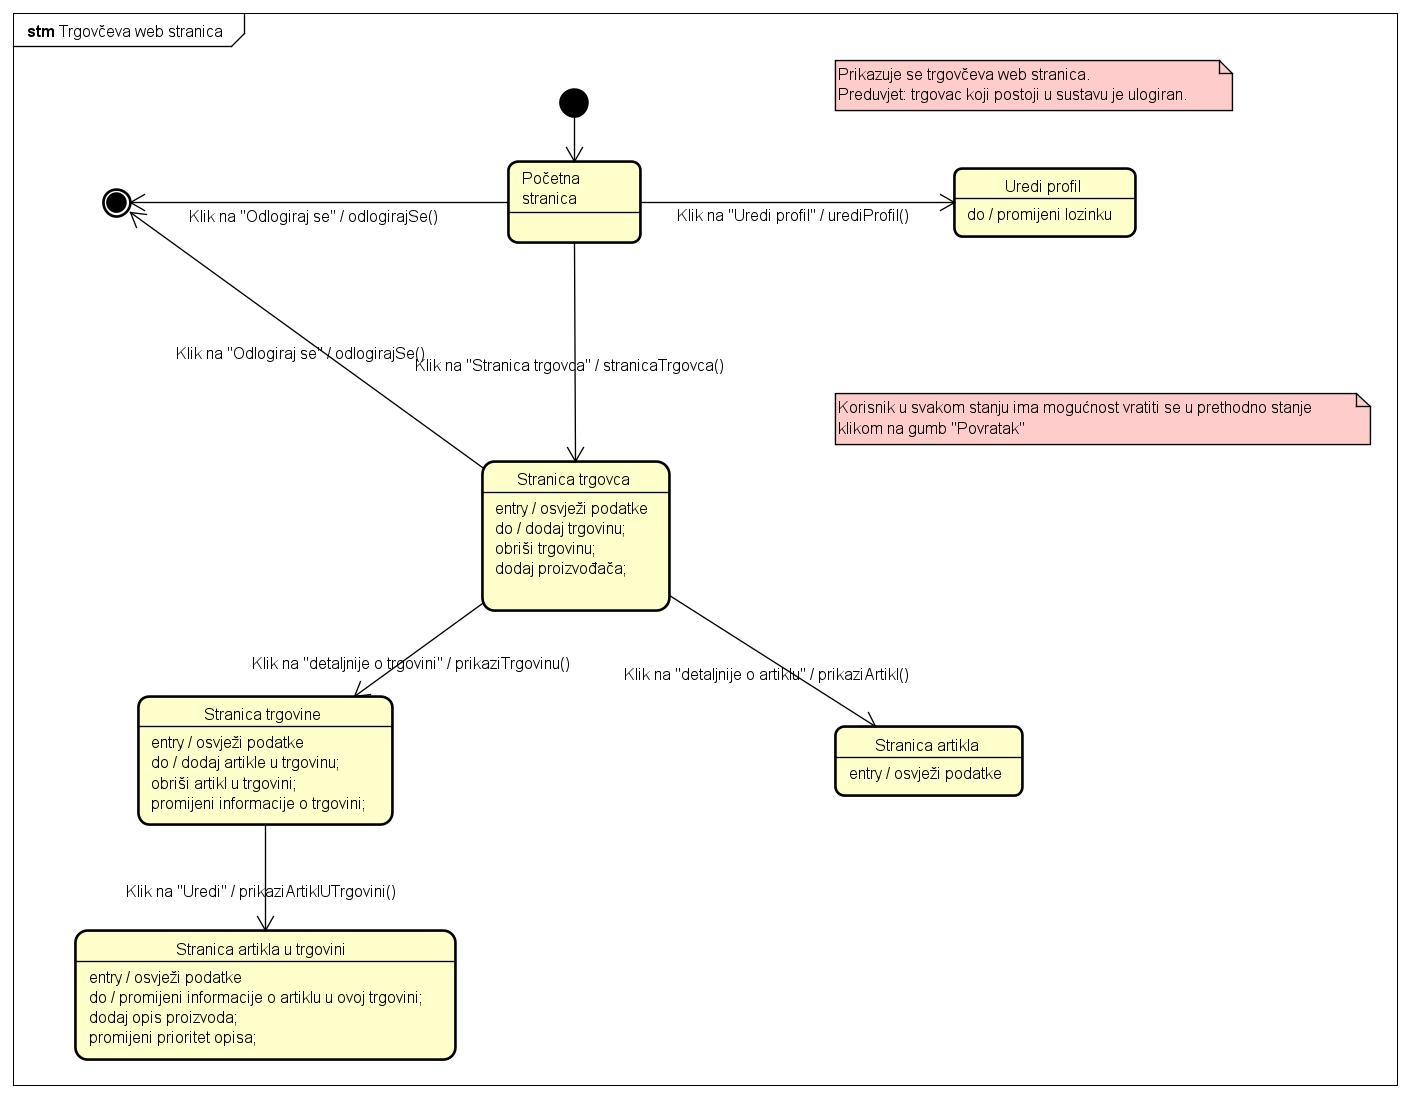
\includegraphics[width=1.0\linewidth]{dijagrami/web-trgovac.jpg}
				\caption{Dijagram stanja web stranice za trgovca}
				\label{fig:state-web-trgovac}
			\end{figure}
			
		
		\section{Dijagram aktivnosti}
			Na slici prikazan je dijagram aktivnosti. On obuhvaća sve aktivnosti koje se događaju na Android aplikaciji, serveru, serverskoj i Android bazi podataka. Obuhvaćeni skup aktivnosti obuhvaća sve od ulogiravanja korisnika na Android uređaju pa do dodavanja artikla na popis.
			
			Korisnik se dakle prvo ulogira, zatim odabere trgovinu te proizvod koji je ponuđen u toj trgovini. Odabirom proizvoda, prikazuje se detaljni opis tog proizvoda, njegova slika te opcije "upvote", "downvote" te "Dodaj na popis". Ovdje sam prikazao postupak dodavanja na popis. Jedan od preduvjeta je taj da postoji barem jedan popis na uređaju.
			
			\begin{figure}[H]
				\centering
				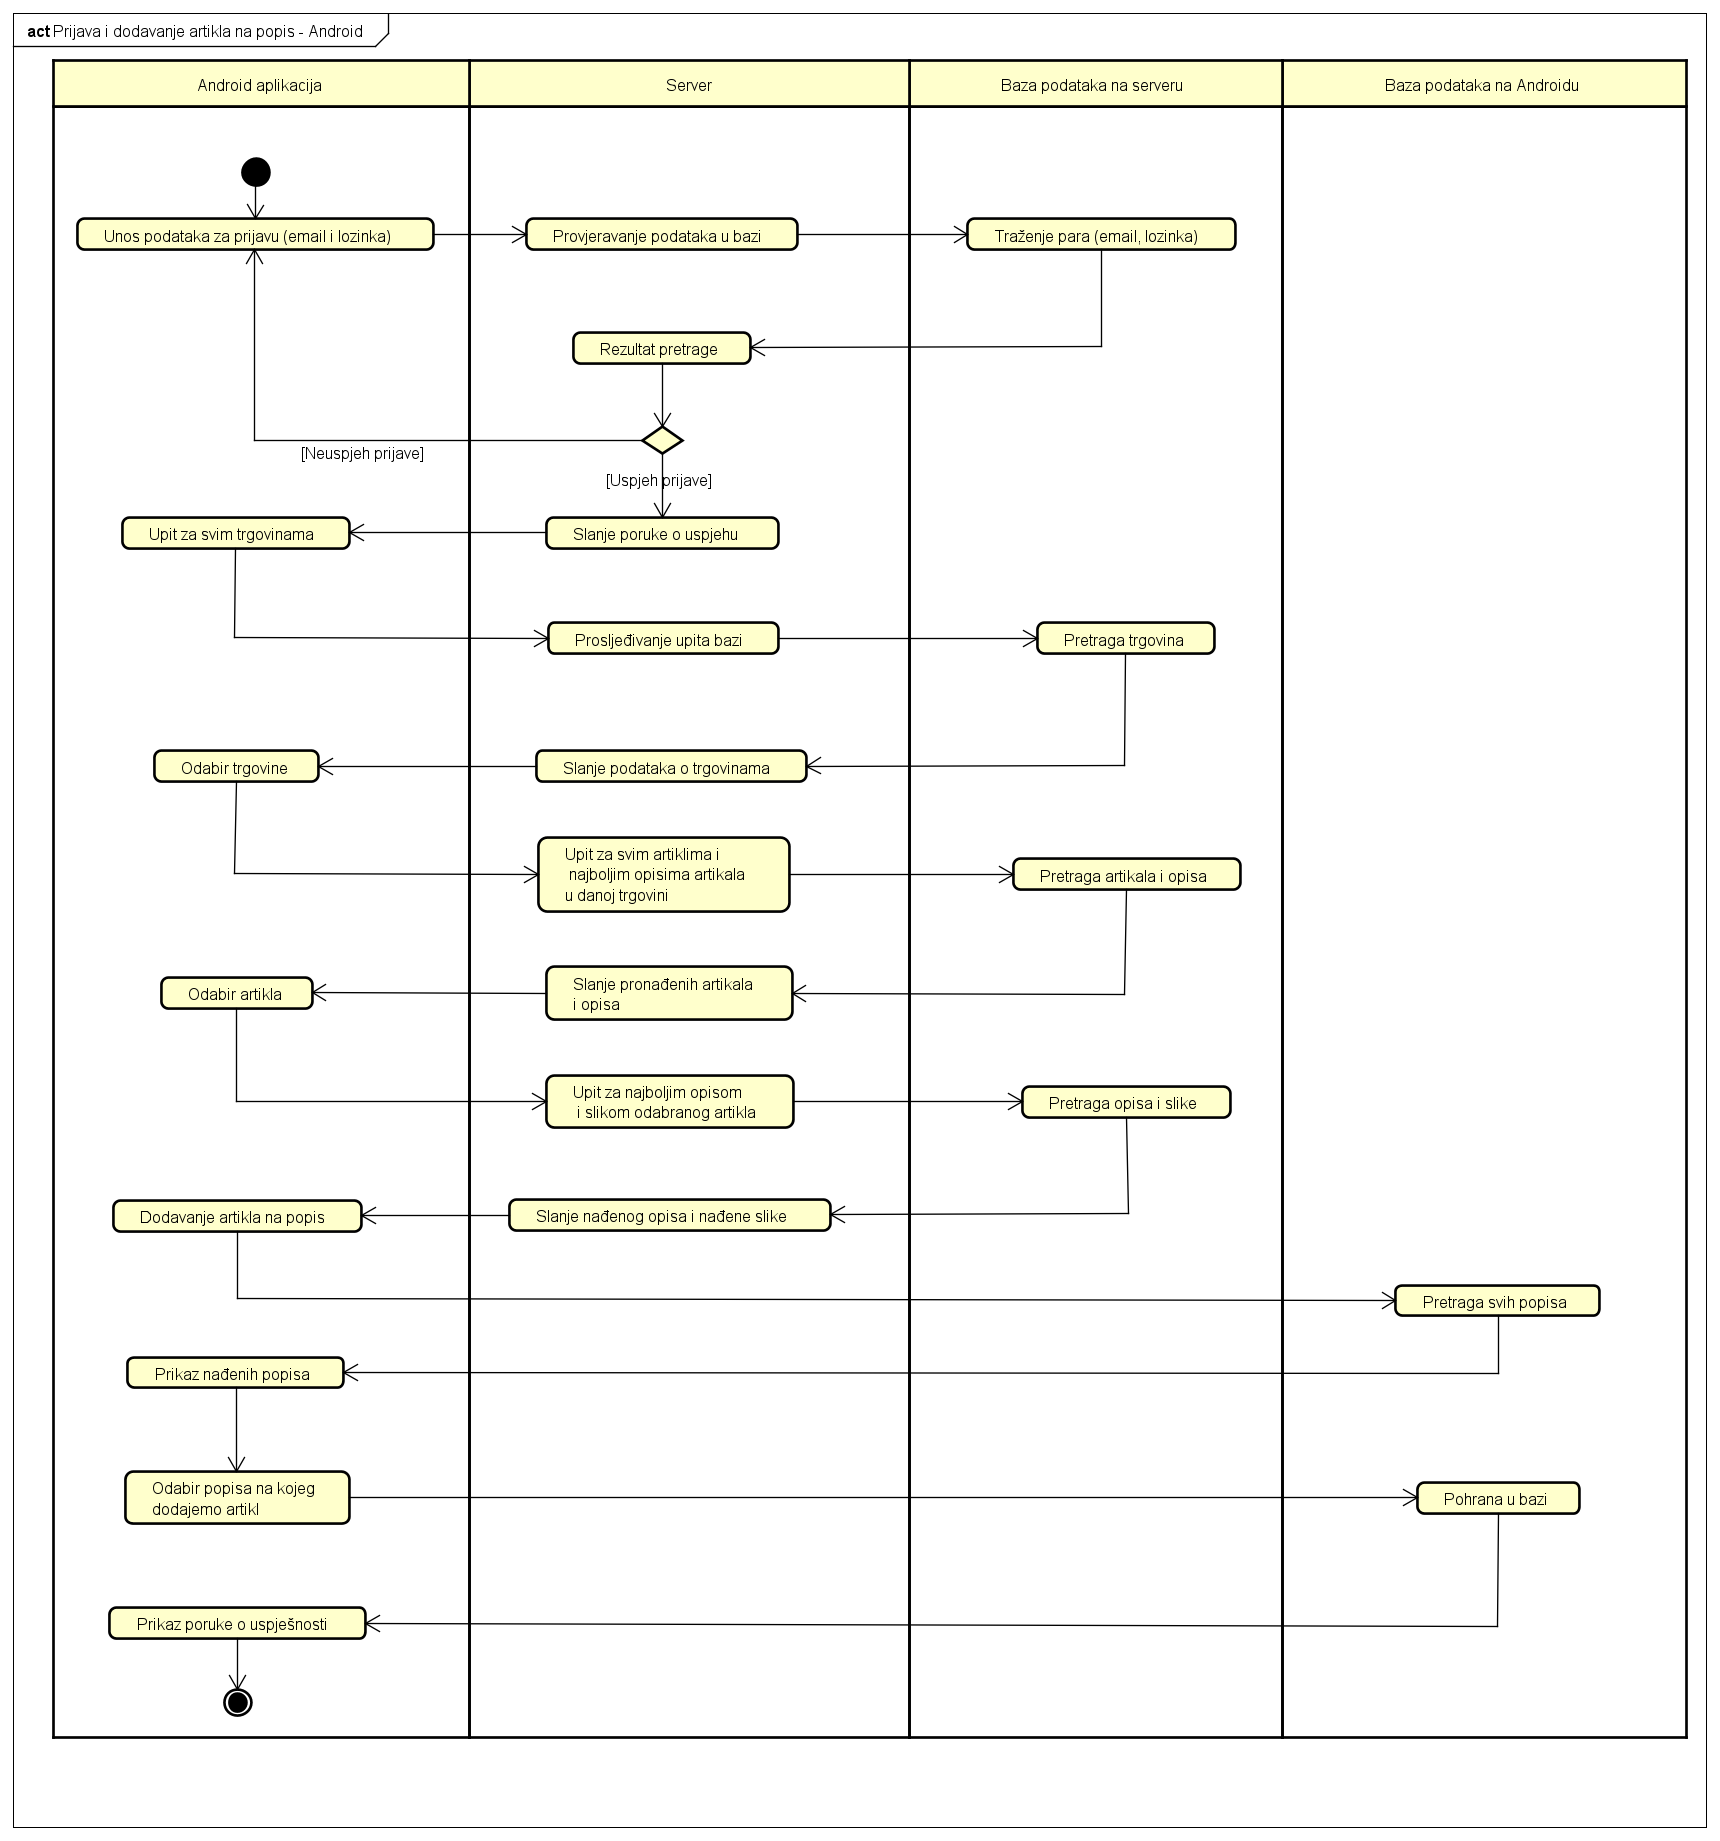
\includegraphics[width=1.0\linewidth]{dijagrami/dodavanje-art.png}
				\caption{Dijagram aktivnosti za prijavu i dodavanje artikla na popis (Android)}
				\label{fig:act-dodavanje-art}
			\end{figure}
		
		\section{Dijagram komponenti}
		
			Dijagram prikazuje komponente aplikacije koje komuniciraju preko sučelja. Web aplikacija od servera, uz podatke u JSON formatu, mora dobiti i izgled stranice - HTML i CSS. Android aplikacija ne traži HTML i CSS zbog toga što je prikaz primljenih podataka od servera (koji se također dobijaju u JSON formatu) definiran na samom Androidu.
			
			Server ima vlastitu bazu podataka s kojom komunicira preko sučelja koje dolazi u paketu Django, a svaki Android uređaj komunicira sa svojom bazom podataka preko sučelja definiranim paketom DBRoom.
			
			Također, Google pruža svoje sučelje koje se može iskoristiti za automatsko slanje mailova. Tu funkcionalnost koristi server kako bi korisniku poslao potvrdu o promjeni lozinke.
		
			\begin{figure}[H]
				\centering
				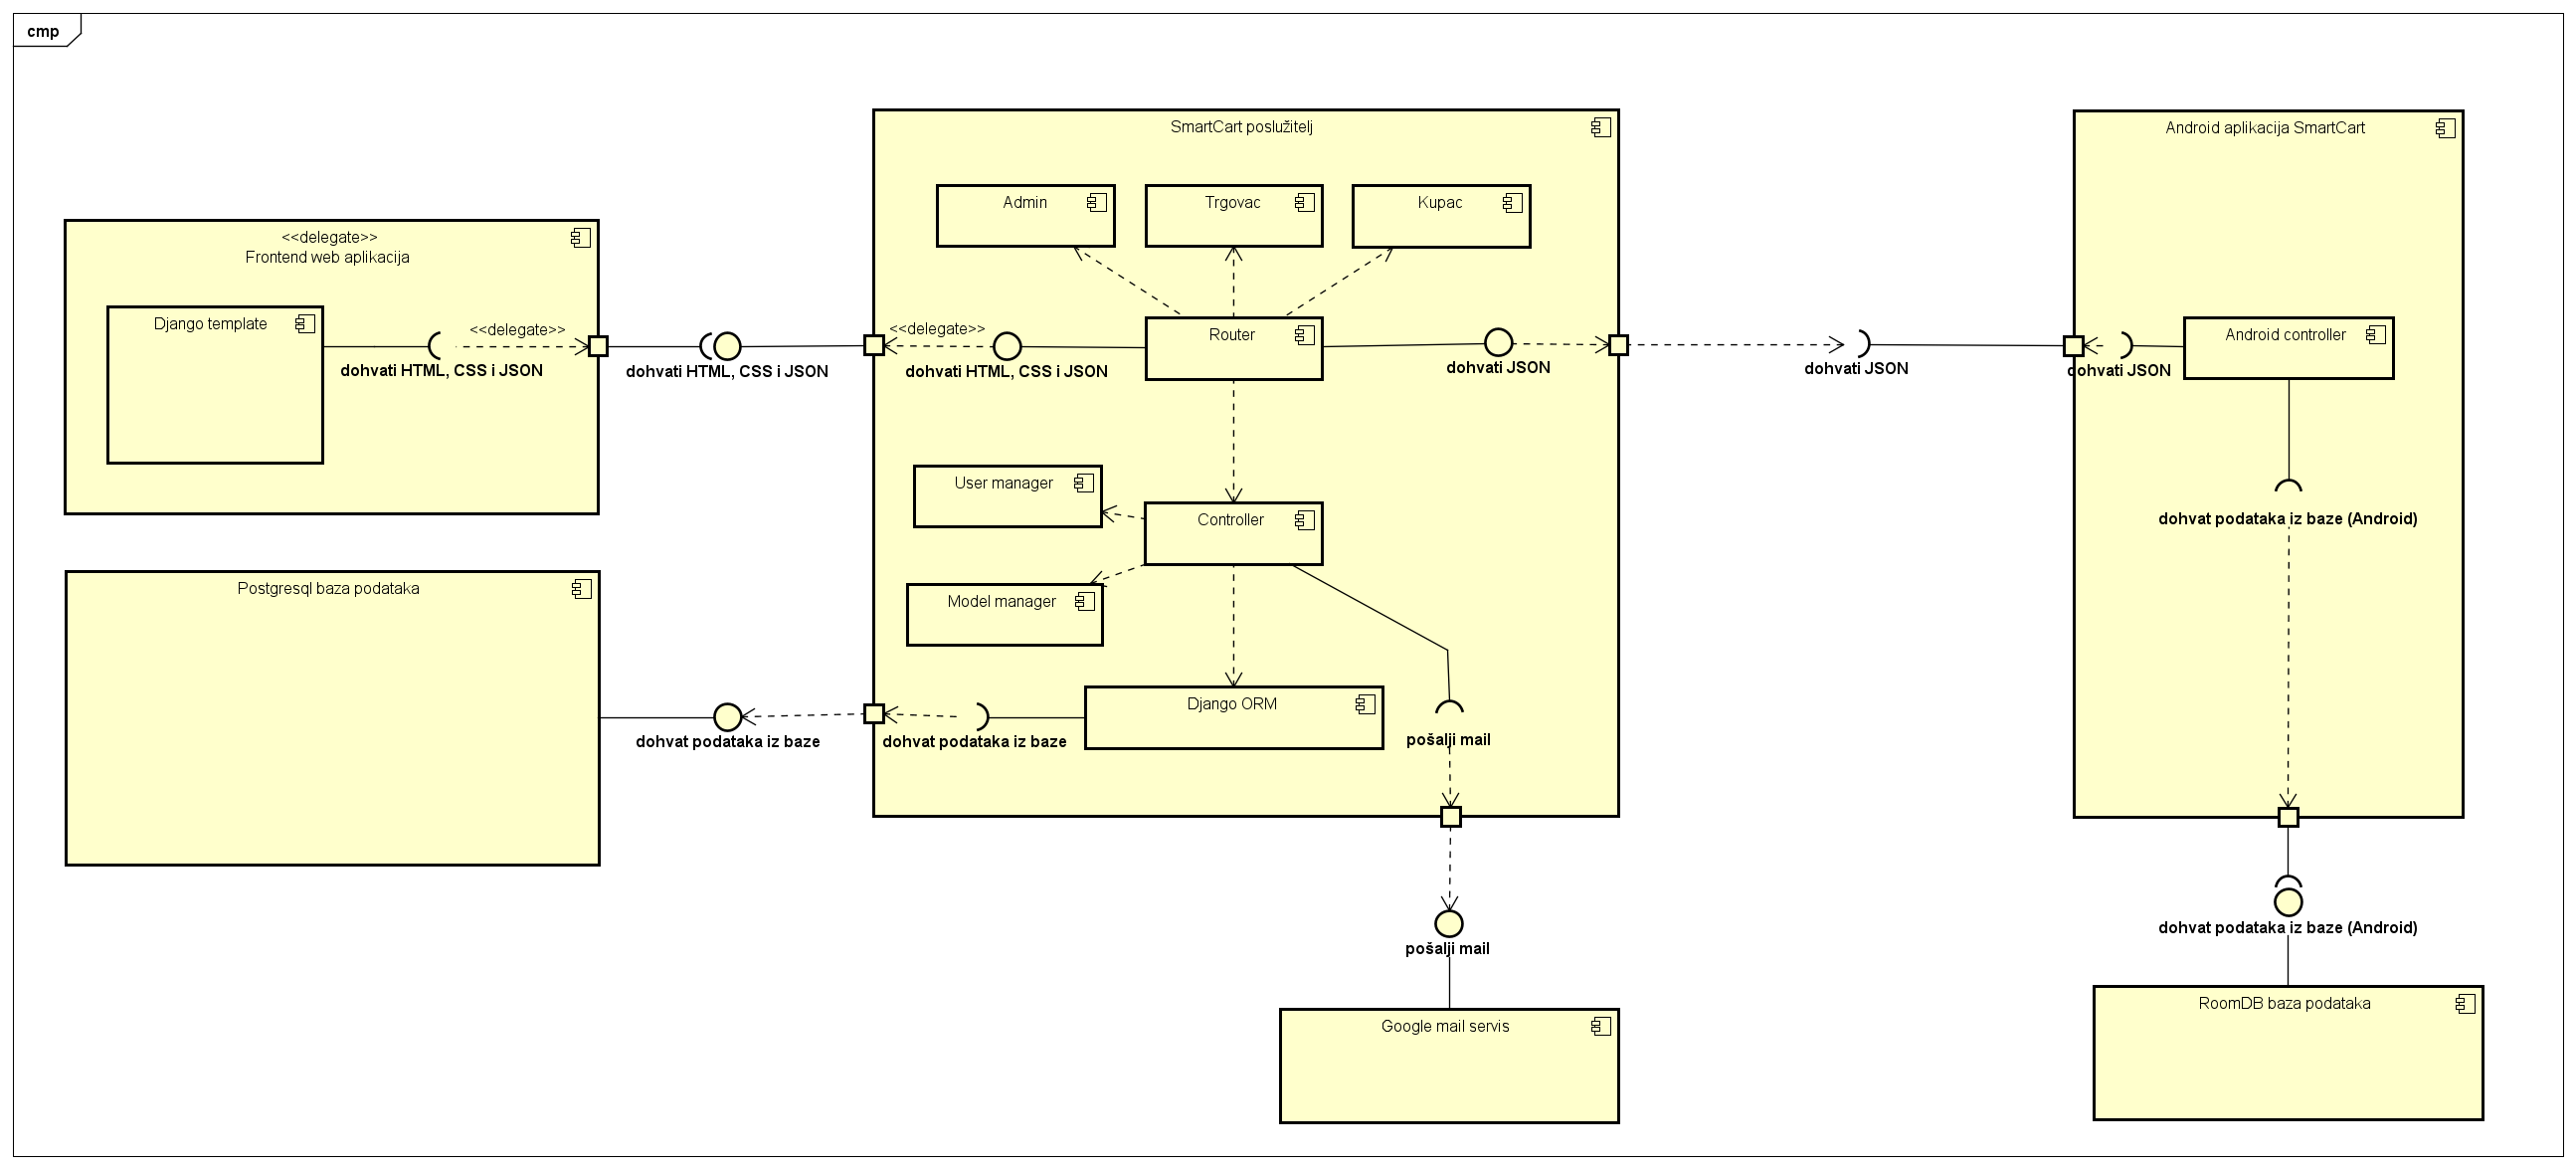
\includegraphics[width=1.0\linewidth]{dijagrami/component.png}
				\caption{Dijagram komponenti}
				\label{fig:cmp-component}
			\end{figure}
			
			
			\eject


	%\chapter{Implementacija i korisničko sučelje}
	\section{Korištene tehnologije i alati}
		Programsko rješenje sastoji se od dva dijela - Android aplikacija i web aplikacija.
		
		Adroid dio pisan je u okruženju AndroidStudio, u nativnom jeziku Java. Za testiranje aplikacije koristili smo ili Android Virtual Device kojeg smo pokretali u okruženju AndroidStudio ili smo aplikaciju direktno instalirali i pokretali na Android uređaju. Baza podataka koju smo koristili za Android je RoomDB koja koristi jezik MySQL.
		
		Web dio pisan je u jeziku Python 3, a korišteni framework je Django. Django omogućava lakše razvijanje i upravljanje bazom podataka, funkcijama kao što su login i logout te nudi dinamičko generiranje HTML stranica. Okruženje koje je smo koristili za razvoj serverskog dijela većinom je ovisilo od osobe do osobe. Neki su preferirali Visual Studio Code, a neki PyCharm, okruženje za Python temeljeno na okruženju IntelliJ. I VSCode i PyCharm nude ugrađene funkcionalnosti za VCS tj. Version Control System.
		
		Baza podataka na serverskom dijelu (tj. glavna baza podataka) je Postgres baza podataka. Korišteni SQL jezik je dakle PostgreSQL, a korišteni DB Manager je pgAdmin.
		
		Komunikacija članova tima je realizirana preko aplikacije Slack i Whatsapp, a samim verzijama koda se upravljalo preko sustava git stranici Gitlab.
		\eject
	\section{Ispitivanje programskog rješenja}
		\subsection{Ispitivanje komponenti}
			
			Budući da ja aplikacija napisana za Android uređaje ispitivanje komponenti
			se provodi pomoću razreda AndroidJUnit4 (\url{https://developer.android.com/reference/androidx/test/ext/junit/runners/AndroidJUnit4})
			uz korištenje funkcionalnosti dostupnih u modulu JUnit5 (\url{https://junit.org/junit5/})
			
			Testiraju se razne funkcionalnosti dostupne na android uređaju, među kojima
			vrijedi izdvojiti testiranje dohvata podataka iz baze podataka na uređaju, testiranje prikazivanja
			stavki na popisu, testiranje prikazivanja popisa, testiranje prikazivanja adrese trgovina i testiranje
			prikazivanja proizvoda
			
			Primjeri testiranja:
			
			\begin{figure}[H]
				\centering
				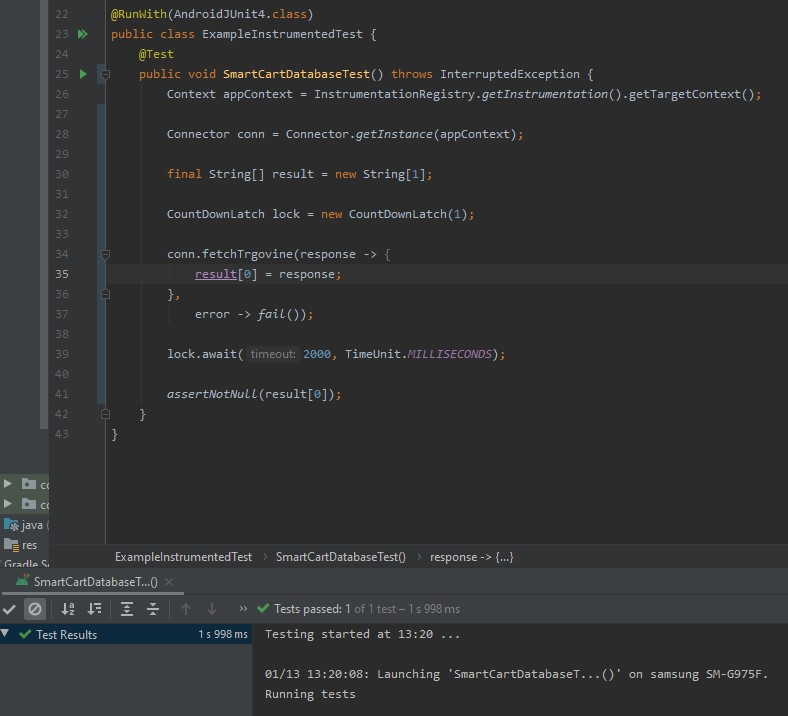
\includegraphics[scale=0.7]{slike/androidTest1.jpg}
				\caption{Testiranje baze podataka na uređaju}
				\label{fig:test_uredaj_db}
			\end{figure}
		
			\begin{figure}[H]
				\centering
				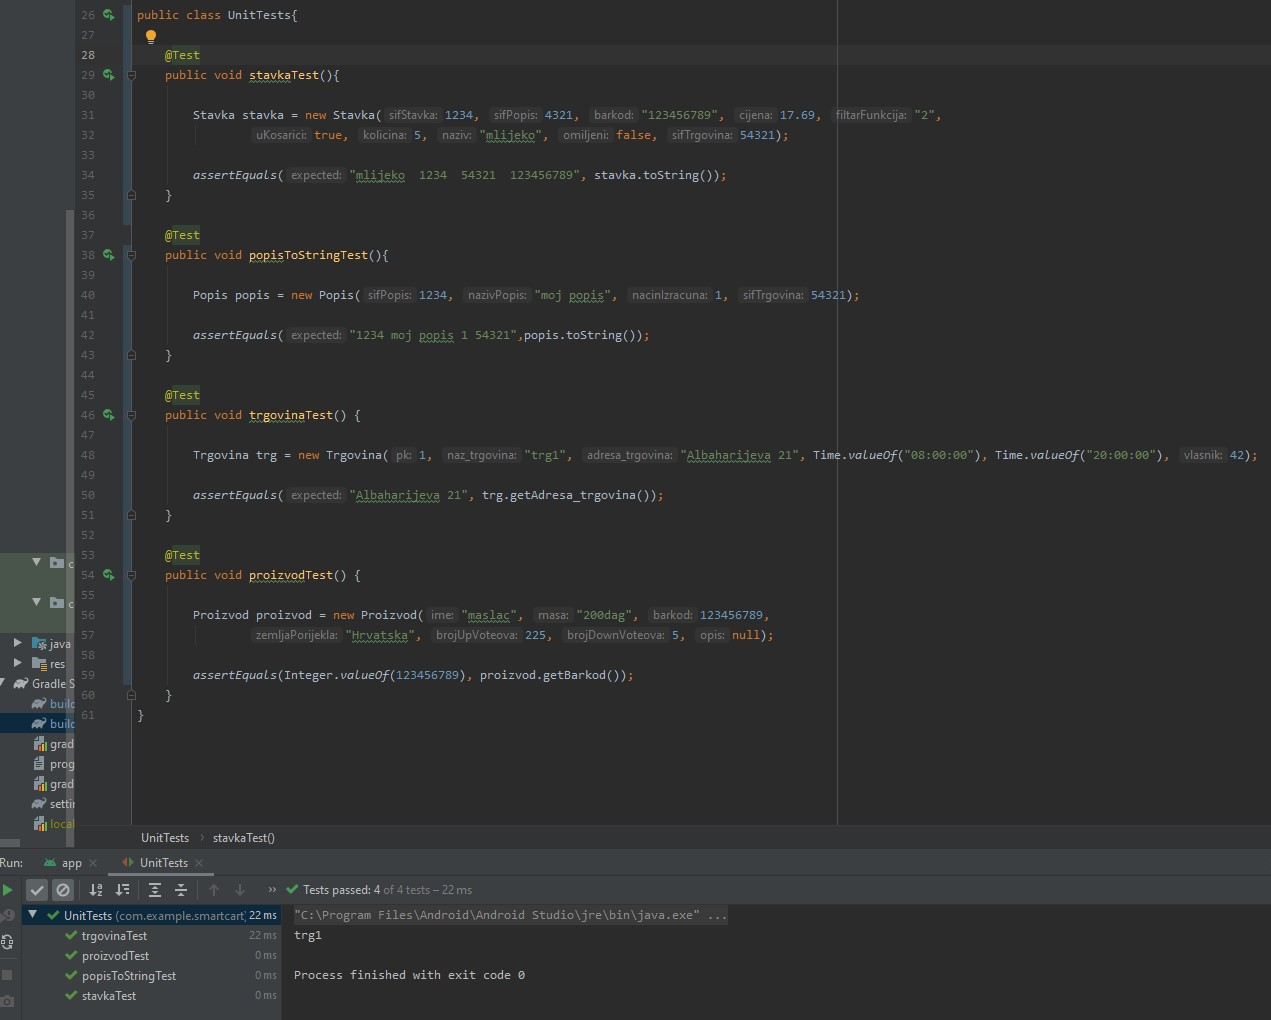
\includegraphics[scale=0.5]{slike/androidTest2.jpg}
				\caption{Testiranje razreda na uređaju}
				\label{fig:test_uredaj_class}
			\end{figure}
		
		\subsection{Ispitivanje sustava}
			
			Ispitivanje sustava je provedeno koristeći funkcionalnosti iz paketa unittest koji dolazi u instalaciji programskog jezika Python u kombinaciji sa alatom Selenium WebDriver koji pruža podršku za automatsko upravljanje internetskim preglednikom. Za instalaciju podrške za ispitivanje sustava potrebno je sa interneta skinuti Selenium za programski jezik Python (\url{https://pypi.org/project/selenium/}, također je moguće instalirati ako se unutar naredbenog retka pozove komanda \textit{pip install selenium}). Uz Selenium za Python potrebno je instalirati i Selenium WebDriver. U našem projektu koristimo geckodriver 0.28.0, verziju Selenium WebDriver-a za internetski preglednik Mozilla Firefox, koja se može skinuti sa sljedeće web-adrese: (\url{https://github.com/mozilla/geckodriver/releases/tag/v0.28.0}).\\
			Nad sustavom se provode razna testiranja. Neka od najvažnijih su:
			
			\begin{itemize}
				\item Testiranje izrade novog profila i pokušaja prijave na web-stranicu pomoću točne i krive kombinacije (relevantan isječak iz koda):
				\lstset{language=Python, tabsize=4, showstringspaces=false, basicstyle=\small}
				\begin{lstlisting}[breaklines]
def fill_login_form(self, username, password):
    self.driver.get(HOME_PAGE)
    self.driver.find_element(By.XPATH, '//button[text()="Log in"]').click()
    self.driver.find_element(By.NAME, "username").send_keys(username)
    self.driver.find_element(By.NAME, "password").send_keys(password)
    self.driver.find_element(By.NAME, "submit_button").click()
					
def test_successful_login(self):
    self.fill_login_form("ante@fer.hr", "pwd")
    self.assertEqual(self.driver.current_url, f"{HOME_PAGE}/trgovac")
					
def test_wrong_login(self):
    self.fill_login_form("ante@fer.hr", "abc")
    self.assertTrue(str(self.driver.current_url).startswith(f"{HOME_PAGE}/login"))
					
def test_create_new_profile(self):
    self.driver.get(HOME_PAGE)
    self.driver.find_element(By.XPATH, '//button[text()="Sign up as kupac"]').click()
    self.driver.find_element(By.NAME, "email").send_keys(NEW_USERNAME)
    self.driver.find_element(By.NAME, "password").send_keys(NEW_PASSWORD)
    self.driver.find_element(By.NAME, "confirm_password").send_keys(NEW_PASSWORD)
    self.driver.find_element(By.NAME, "submit_button").click()
    self.fill_login_form(NEW_USERNAME, NEW_PASSWORD)
    self.assertTrue(f"Logged in as {NEW_USERNAME}" in self.driver.page_source)	
				\end{lstlisting}
				\item Testiranje dodavanja novog proizvoda (relevantan isječak iz koda):
				\begin{lstlisting}[breaklines]
def test_adding_new_barcode(self):
	self.fill_login_form("ante@fer.hr", "pwd")
	self.driver.find_element(By.NAME, "barkod_artikla").send_keys(BARCODE)
	self.driver.find_element(By.NAME, "new_barcode_button").click()
	list_of_products = self.driver.find_element(By.ID, "products")
	self.assertTrue(BARCODE in list_of_products.text)
				\end{lstlisting}
				\item Testiranje „sigurnosti“ stranice (nepostojeći linkovi i pristup linkovima koji zahtjevaju posebnu dozvolu) (relevantan isječak iz koda):
				\begin{lstlisting}[breaklines]
def test_wrong_link(self):
	self.driver.get(f"{HOME_PAGE}/another_link/that_doesnt_exist")
	self.assertEqual(self.driver.current_url, f"{HOME_PAGE}/")

def test_page_permissions(self):
	self.fill_login_form(NEW_USERNAME, NEW_PASSWORD)
	self.driver.get(f"{HOME_PAGE}/trgovac")
	self.assertEqual(self.driver.current_url, f"{HOME_PAGE}/")
				\end{lstlisting}
			\end{itemize}
		
			Razultati testiranja:
			\begin{figure}[H]
				\centering
				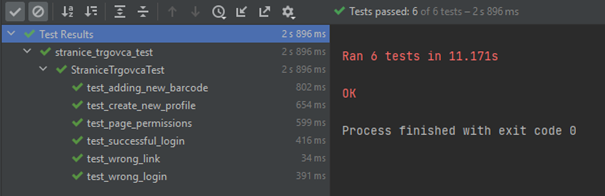
\includegraphics{slike/serverTest.png}
				\caption{Razultati testiranja servera}
				\label{fig:test_server}
			\end{figure}
		\eject
	\section{Dijagram razmještaja}
			Server, i serverska baza podataka nalaze se na jednom računalu. Korisnik ima nekoliko opcija ako želi pristupiti aplikaciji. Korisni može web aplikaciji pristupiti iz bilo kojeg web preglednika. Nadalje, korisnik može aplikaciji pristupiti i preko Android uređaja na kojem je instalirao SmartCart aplikaciju. Android aplikacija, kao i web aplikacija, komunikaciju sa serverom obavljaju HTTP protokolom.
		
			\begin{figure}[H]
				\centering
				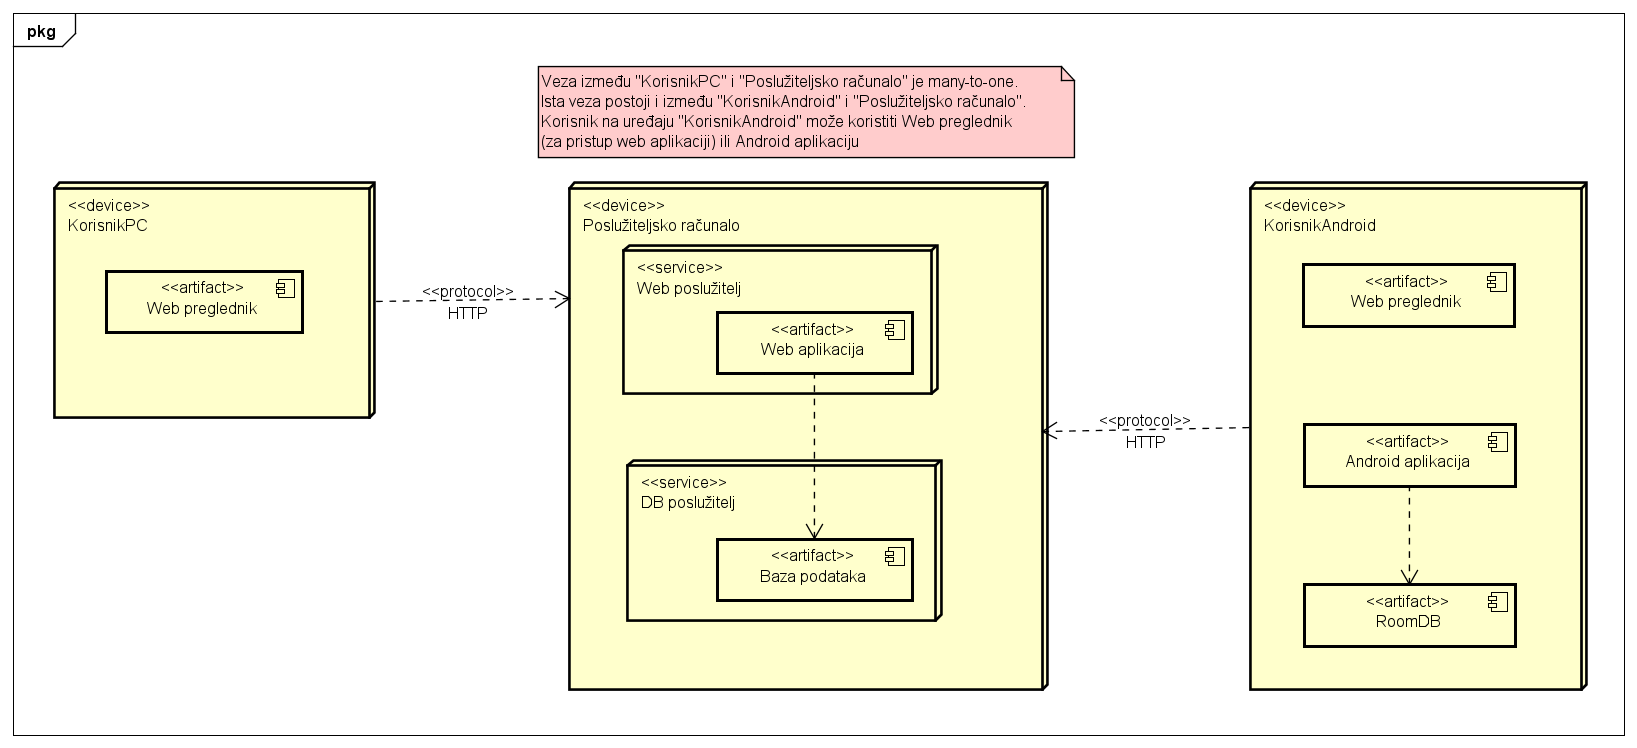
\includegraphics[width=1.0\linewidth]{dijagrami/deployment.png}
				\caption{Dijagram razmještaja}
				\label{fig:deployment}
			\end{figure}
		\eject
	\section{Upute za puštanje u pogon}
		Ovo treba napisati.
		\eject
			
	%\chapter{Zaključak i budući rad}
	Ovo treba napisati
	\eject
	\chapter*{Popis literature}
		\addcontentsline{toc}{chapter}{Popis literature}
		
		
		\begin{enumerate}
			
			\item  StackOverflow, \url{https://stackoverflow.com/}
			
			\item  Programsko inženjerstvo, FER ZEMRIS, \url{http://www.fer.hr/predmet/proinz}
		
			
			%\item  I. Sommerville, "Software engineering", 8th ed, Addison Wesley, 2007.
			
			%\item  T.C.Lethbridge, R.Langaniere, "Object-Oriented Software Engineering", 2nd ed. McGraw-Hill, 2005.
			
			%\item  I. Marsic, Software engineering book``, Department of Electrical and Computer Engineering, Rutgers University, \url{http://www.ece.rutgers.edu/~marsic/books/SE}
			
			\item  The Unified Modeling Language, \url{https://www.uml-diagrams.org/}
			
			\item  Astah Community, \url{http://astah.net/editions/uml-new}
		\end{enumerate}
		
		 

	
	
	\begingroup
	\renewcommand*\listfigurename{Indeks slika i dijagrama}
	%\renewcommand*\listtablename{Indeks tablica}
	%\let\clearpage\relax
	\listoffigures
	%\vspace{10mm}
	%\listoftables
	\endgroup
	\addcontentsline{toc}{chapter}{Indeks slika i dijagrama}


	
	\eject 
		
	\chapter*{Dodatak: Prikaz aktivnosti grupe}
		\addcontentsline{toc}{chapter}{Dodatak: Prikaz aktivnosti grupe}
		
		\section*{Dnevnik sastajanja}
		
		\begin{packed_enum}
			\item  sastanak
			\item[] \begin{packed_item}
				\item Datum: 14. listopada 2020.
				\item Prisustvovali: cijeli PreljevStoga
				\item Teme sastanka:
				\begin{packed_item}
					\item  diskusija zadatka
					\item  upoznavanje s git-om i GitLab-om
				\end{packed_item}
			\end{packed_item}
			
			\item  sastanak
			\item[] \begin{packed_item}
				\item Datum: 15. listopada 2020.
				\item Prisustvovali: dr.sc.M.Krhen, I.Rissi, cijeli PreljevStoga
				\item Teme sastanka:
				\begin{packed_item}
					\item  diskutiranje zadatka koji si je grupa zadala
					\item  savjeti za rad na projektu
				\end{packed_item}
			\end{packed_item}
			
			\item  sastanak
			\item[] \begin{packed_item}
				\item Datum: 22. listopada 2020.
				\item Prisustvovali: dr.sc.M.Krhen, I.Rissi, D.Grubelić, J.Komljenović, A.Lakoš, L.Pranjić, M.Vladić
				\item Teme sastanka:
				\begin{packed_item}
					\item  upit vezan uz ispravno pisanje dokumentacije
				\end{packed_item}
			\end{packed_item}
			
			\item  sastanak
			\item[] \begin{packed_item}
				\item Datum: 24. listopada 2020.
				\item Prisustvovali: cijeli PreljevStoga
				\item Teme sastanka:
				\begin{packed_item}
					\item  odabir tehnologija
					\item  raspoređivanje poslova
					\item  definiranje zadataka za naredni tjedan
				\end{packed_item}
			\end{packed_item}
			
			\item  sastanak
			\item[] \begin{packed_item}
				\item Datum: 28. listopada 2020.
				\item Prisustvovali: T.Bjelčić, D.Grubelić, J.Komljenović, A.Lakoš, L.Pranjić, M.Vladić
				\item Teme sastanka:
				\begin{packed_item}
					\item  demonstracija prve inačice dokumentacije
					\item  definiranje strukture git \textit{repositoryja} i raščišćavanje drugih nedoumica oko git-a
					\item  priprema za izradu temeljne inačice Android dijela aplikacije
					\item  definiranje daljnjeg rasporeda poslova
				\end{packed_item}
			\end{packed_item}
			
			\item  sastanak
			\item[] \begin{packed_item}
				\item Datum: 29. listopada 2020.
				\item Prisustvovali: D.Grubelić, J.Komljenović, A.Lakoš
				\item Teme sastanka:
				\begin{packed_item}
					\item  demonstracija rada s djangom J.Komljenovića
				\end{packed_item}
			\end{packed_item}
			
			\item  sastanak
			\item[] \begin{packed_item}
				\item Datum: 29. listopada 2020.
				\item Prisustvovali: dr.sc.M.Krhen, I.Rissi, T.Bjelčić, D.Grubelić, J.Komljenović, A.Lakoš, L.Pranjić, M.Vladić
				\item Teme sastanka:
				\begin{packed_item}
					\item  dogovor oko izmjene funkcionalnih zahtjeva
					\item  upit vezan uz pravilan izgled UML dijagrama
				\end{packed_item}
			\end{packed_item}
			
			\item  sastanak
			\item[] \begin{packed_item}
				\item Datum: 1. studenog 2020.
				\item Prisustvovali: T. Bjelčić, D.Grubelić, J.Komljenović, A.Lakoš, M.Vladić
				\item Teme sastanka:
				\begin{packed_item}
					\item  demonstracija napretka na backend dijelu
					\item  dogovor oko daljnjeg rasporeda poslova
				\end{packed_item}
			\end{packed_item}
			
			\item  sastanak
			\item[] \begin{packed_item}
				\item Datum: 2. studenog 2020.
				\item Prisustvovali: T.Bjelčić, D.Grubelić, J.Komljenović, A.Lakoš, L.Pranjić, M.Vladić
				\item Teme sastanka:
				\begin{packed_item}
					\item  rasprava o budućim planovima s obzirom na zadaće iz drugog predmeta
					\item  dogovor o prebacivanju SQL upita o artiklima i trgovinama na poslužitelj
				\end{packed_item}
			\end{packed_item}
			
			\item  sastanak
			\item[] \begin{packed_item}
				\item Datum: 6. studenog 2020.
				\item Prisustvovali: cijeli PreljevStoga
				\item Teme sastanka:
				\begin{packed_item}
					\item  dogovor oko opsega generičkih funkcionalnosti za prvu predaju
					\item  raspored poslova
					\item  kratki prolazak kroz dokumentaciju
				\end{packed_item}
			\end{packed_item}
			
			%
			
		\end{packed_enum}
		
		\eject
		\section*{Tablica aktivnosti}
		    \begin{longtabu} to \textwidth {|X[7, l]|X[1, c]|X[1, c]|X[1, c]|X[1, c]|X[1, c]|X[1, c]|X[1, c]|}
								
				\cline{2-8} \multicolumn{1}{c|}{\textbf{}} &     \multicolumn{1}{c|}{\rotatebox{90}{\textbf{Tomislav Bjelčić }}} & \multicolumn{1}{c|}{\rotatebox{90}{\textbf{Dominik Brdar }}} &	\multicolumn{1}{c|}{\rotatebox{90}{\textbf{Damjan Grubelić }}} &	\multicolumn{1}{c|}{\rotatebox{90}{\textbf{Josip Komljenović }}} &
				\multicolumn{1}{c|}{\rotatebox{90}{\textbf{Antonio Lakoš }}} &
				\multicolumn{1}{c|}{\rotatebox{90}{\textbf{Luka Pranjić }}} &	\multicolumn{1}{c|}{\rotatebox{90}{\textbf{Marko Vladić }}} \\ \hline 
				\endfirsthead
				
			
				\cline{2-8} \multicolumn{1}{c|}{\textbf{}} &     \multicolumn{1}{c|}{\rotatebox{90}{\textbf{Tomislav Bjelčić}}} & \multicolumn{1}{c|}{\rotatebox{90}{\textbf{Dominik Brdar }}} &	\multicolumn{1}{c|}{\rotatebox{90}{\textbf{Damjan Grubelić }}} &
				\multicolumn{1}{c|}{\rotatebox{90}{\textbf{Josip Komljenović }}} &	\multicolumn{1}{c|}{\rotatebox{90}{\textbf{Antonio Lakoš }}} &
				\multicolumn{1}{c|}{\rotatebox{90}{\textbf{Luka Pranjić }}} &	\multicolumn{1}{c|}{\rotatebox{90}{\textbf{Marko Vladić }}} \\ \hline 
				\endhead
				
				
				\endfoot
							
				 
				\endlastfoot
				
				Upravljanje projektom 		& 5 &  & 3 & 2 & 5 & 3 & \\ \hline
				Opis projektnog zadatka 	& 6 & 1 & 3 &  & 12 & 5 & 2 \\ \hline
				
				Funkcionalni zahtjevi       & 5 & 1 & 2 & 3 & 2 & 3 & 2 \\ \hline
				Opis pojedinih obrazaca 	&  &  & 24 &  & 3 &  &  \\ \hline
				Dijagram obrazaca 			&  & 1 & 5 &  & 3 & 2 &  \\ \hline
				Sekvencijski dijagrami 		&  & 2 & 4 &  &  &  &  \\ \hline
				Opis ostalih zahtjeva 		&  & 1 & 1 &  & 2 &  & 1 \\ \hline

				Arhitektura i dizajn sustava	 & 2 & 1 & 2 &  &  & 4 & 2 \\ \hline
				Baza podataka				&  & 3 & 4 & 5 &  &  &   \\ \hline
				Dijagram razreda 			&  &  &  &  &  & 4 &  2 \\ \hline
				Dijagram stanja				&  &  &  &  &  &  &  \\ \hline
				Dijagram aktivnosti 		&  &  &  &  &  &  &  \\ \hline
				Dijagram komponenti			&  &  &  &  &  &  &  \\ \hline
				Korištene tehnologije i alati 		& 4 & 2 &  &  & 3 & 7 &  2\\ \hline
				Ispitivanje programskog rješenja 	& 5 & 12 & 4 & 2 & 15 & 3 &  \\ \hline
				Dijagram razmještaja			&  &  &  &  &  &  &  \\ \hline
				Upute za puštanje u pogon 		&  &  &  &  & 1 &  &  \\ \hline 
				Dnevnik sastajanja 			& 3 & 1 & 1 &  & 1 &  & 1 \\ \hline
				Zaključak i budući rad 		&  &  &  &  &  &  &  \\  \hline
				Popis literature 			&  &  &  &  &  &  &  \\  \hline
				&  &  &  &  &  &  &  \\ \hline \hline
				Demonstracija nove tehnologije &  &  & 3 &  &  &  &  \\ \hline
				Back end     		        &  & 13 & 1 & 30 & 25 & 2 & 18 \\ \hline 
				Dizajn sučelja              & 8 &  & 2 & 1 & 1 & 6 & 5 \\ \hline
				Front end              & 19 & 3 & 11 & 3 & 4 & 21 & 23 \\ \hline
				
				
			\end{longtabu}
					
					
		\eject
		
	



\end{document} %naredbe i tekst nakon ove naredbe ne ulaze u izgrađen dokument 


